% !TEX root = ../notes_template.tex
\chapter{Ventilation}\label{chp:alveolar_oxygen}
Updated on \today
\minitoc

Oxygen intake and carbon dioxide output are necessary for skeletal muscle energetics. Sustaining a flow of $O_2$ into the mitochondria requires the intake of $O_2$ by drawing air into the lungs (ventilation) and the alveoli (alveolar ventilation). Similarly, the flow of $CO_2$ out of the mitochrondria requires expiring $CO_2$ out of the alveoli and lungs. This chapter covers alveolar ventilation ($V_A$), ventilation ($V_e$), ventilation/perfusion ($V/Q$) matching, the regulation of respiration through ventilation, and an introduction to several practice considerations.

\vspace{5mm}

\textbf{Objectives (reluctantly) included:}
\begin{enumerate}
    \item Explain the relationship between ventilation, alveolar ventilation and ventilation/perfusion matching (assumes you know what all of these things are and factors that influence them which are covered throughout the entire chapter not just the overview).
    \item Explain the airways of ventilation.
    \item Explain the impact of breathing pattern on anatomical dead space.
    \item Explain bronchopulmonary hygiene and airway clearance.
    \item Explain the benefit of breathing through the nasal passageways.
    \item Explain bronchodilation and bronchoconstriction.
    \item Explain ventilation volumes and capacities including the connection to the thorax and relate to chest wall excursion as ROM
    \item Explain the mechanics of the ventilatory pump (Section 10.4)
    \item Explain ventilation regulation (Section 10.6)
    \item Explain practice considerations of ventilation (Section 10.7)
    \item Integrate the concepts of this chapter with those of the Respiration and Circulation Chapters.
\end{enumerate}

As you can see - these boil down to one objective. Know and understand the material in this chapter to the extent of being able to explain the concepts. But also to be able to integrate the concepts in this chapter with the Respiration and Circulation chapters (minimally).

\section{Ventilation Overview}

Chapter \ref{chp:blood_oxygen} on Respiration established the need for alveolar ventilation and alveolar circulation. There are three recurring and important preliminary concepts: alveolar ventilation ($V_A$), ventilation ($V_e$) and ventilation / perfusion matching ($V/Q$).

\subsection{Important Preliminary Concept}

\begin{itemize}
    \item Alveolar ventilation ($V_A$) is the movement of air into, and out of, the alveoli. Without continuous $V_A$ there is no alveolar respiration. 
    \item $V_e$ is the movement of air into, and out of, the lungs. $V_e$ is necessary for $V_A$. Without ventilation ($V_e$), there is no $V_A$. \item Pulmonary perfusion is based on circulation ($Q$) and must be primarily distributed to alveoli receiving alveolar ventilation ($V_A$). $V/Q$ matching refers to the matching of $V_A$ and pulmonary circulation ($Q$). Both $V_A$ and $Q$ are necessary for alveolar respiration. Without $V_A$ matching with pulmonary $Q$ there is no alveolar respiration.
 \end{itemize}

$V_e$ is the volume of air inspired (breathe in) or expired (breathe out) in a time period. It is most commonly measured in $mL/min$ or $L/min$. As a volume per minute, it is the volume of air per breath times the number of breaths per minute (bpm):
\vspace{3mm}
\begin{equation}
    V_e (mL/min) = V_t (mL) \times RR (bpm)
    \label{Ve}
\end{equation}
\vspace{3mm}

In Equation \ref{Ve}, the abbreviation $V_t$ stands for tidal volume. Tidal volume is the volume of air inspired (or expired) with one breath. The underlying assumption for both $V_e$ and $V_t$ is that the volume of air inspired equals the volume of air expired. While this might not be the case breath by breath, it is the case over a minute (or longer) time periods.\footnotemark\footnotetext{I've avoided analogies between ventilation and cardiac output for the sake of space and time. However, for those inclined to look for them, you'll find them.}

\paragraph{} If there is an imbalance between $V_t$ in and $V_t$ out, it tends to be limited to transient periods that involve dynamic changes in $V_t$. For example, when $V_t$ increases in the transient periods from rest to exercise, or during exercise when there are variations in $O_2$ needs.

\paragraph{Question:} What would happen if the volume inspired did not equal the volume expired over a long period of time? Try this, breathe more in than out, how long can you do that? Now breathe more out than in, how long can you do that?

\paragraph{Not all $V_e$ ends in the alveoli ($V_A$)}, either per breath ($V_t$), or per minute ($V_e$). And, not all $V_A$ is going to be to alveoli with perfusion (receive capillary circulation). Figure \ref{fig:ve_va.jpg} depicts the general concept that $V_e$ is going to be greater than $V_A$; and that $V_A$ is going to be greater than the $V/Q$. Pulmonary regulation is largely based on minimizing the discrepancy between $V_e$, $V_A$ and $V/Q$.

\begin{figure}
    \centering
    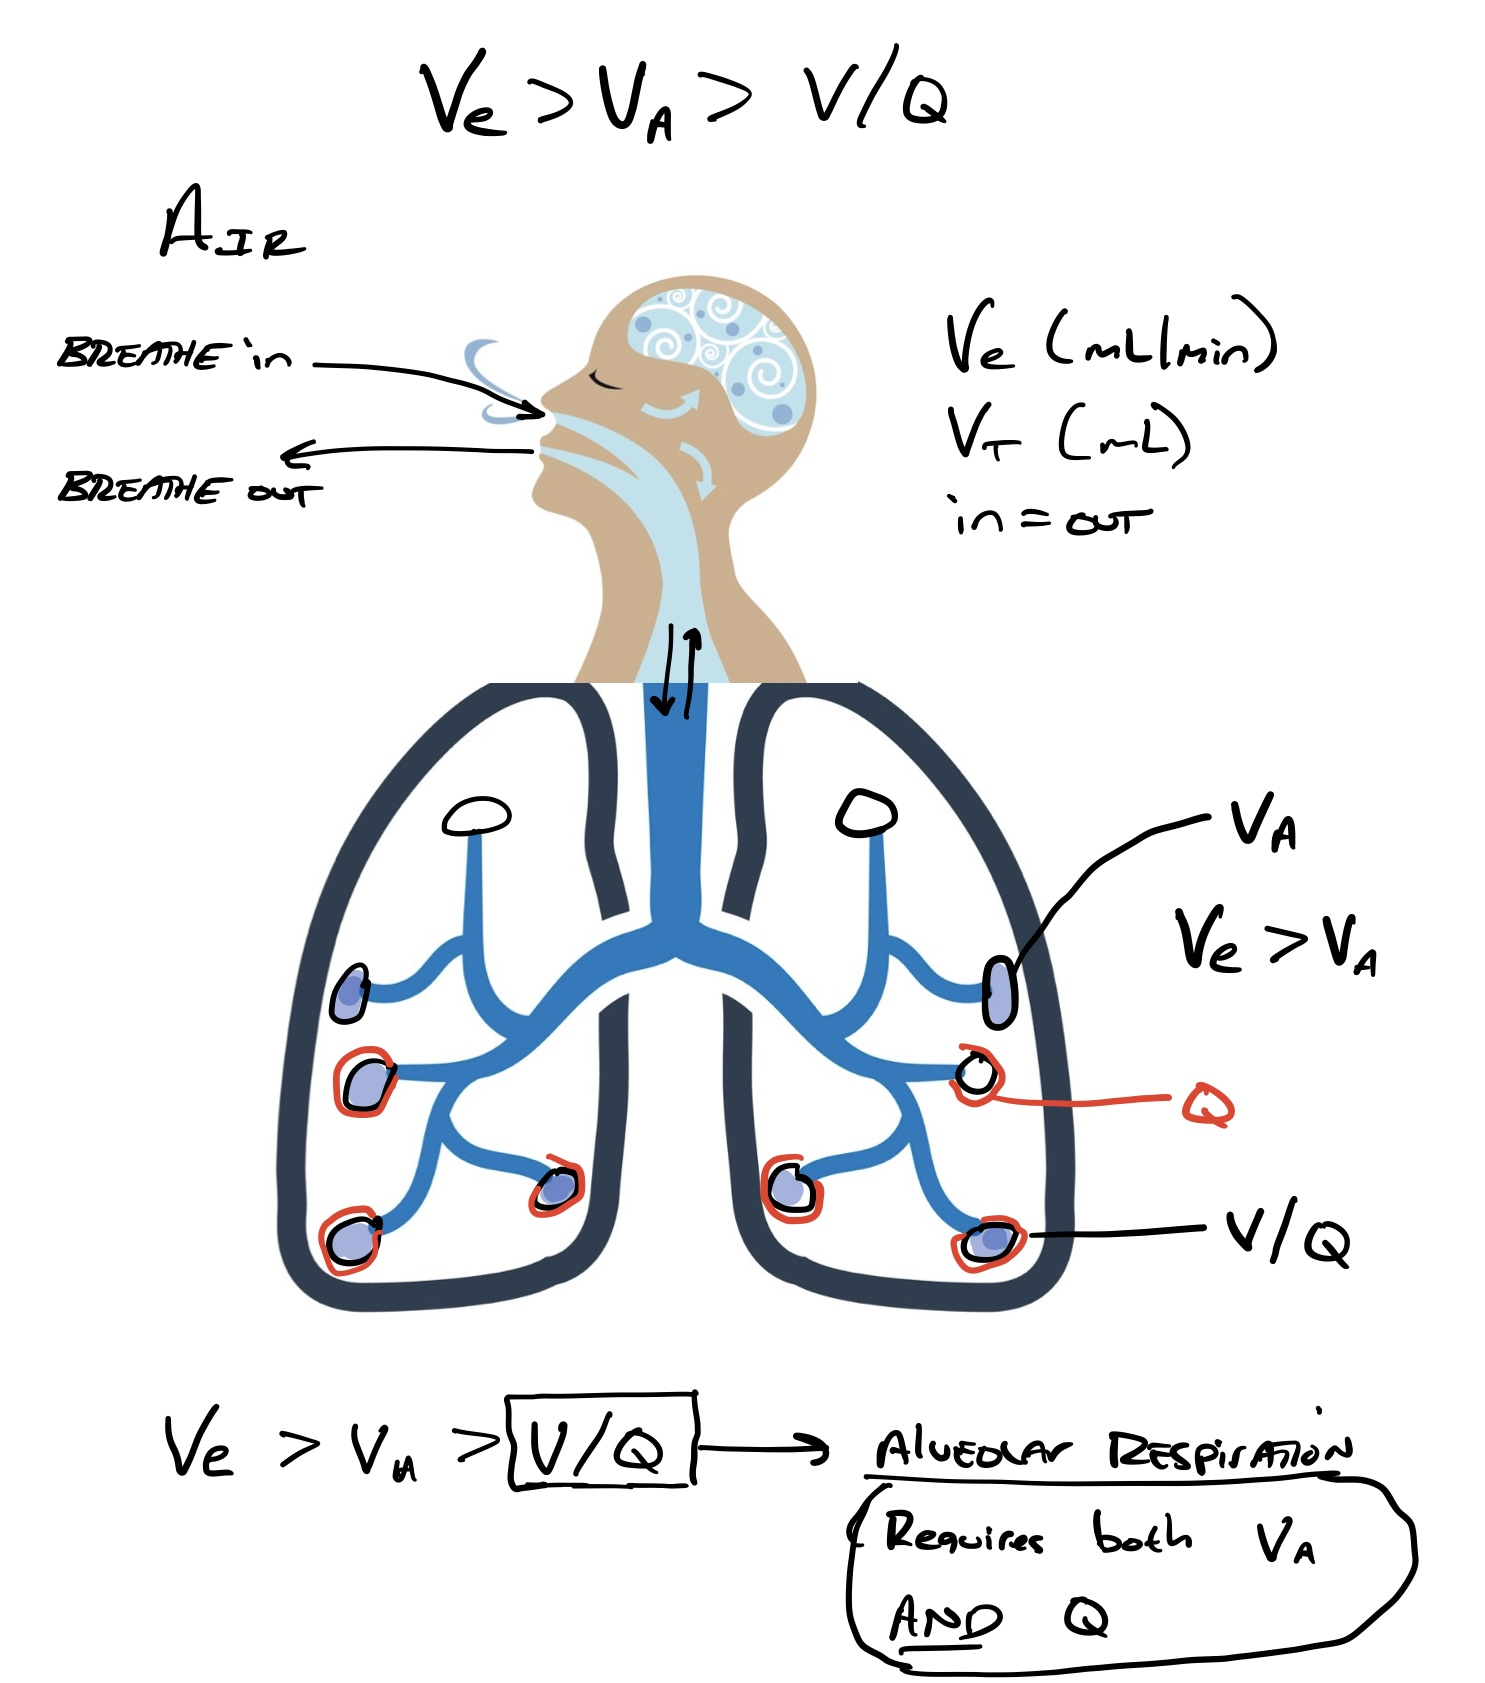
\includegraphics[width = 0.5\linewidth]{./figure/ventilation/ve_va.jpg}
    \caption{Ventilation \& Alveolar Ventilation (Draft)}
    \label{fig:ve_va.jpg}
\end{figure}

\paragraph{The importance of this concept} is that the alveolar respiration relies on the match between alveolar ventilation ($V_A$) and perfusion ($Q$). The consequences of all pulmonary (lung), and many cardiovascular conditions, ultimately rest on how they impact the ability to ventilate ($V_e$), the ability to turn as much $V_e$ into alveolar ventilation ($V_A$) as possible, or the ability to have as much $V_A$ perfusion as possible. Take home message: Many cardiopulmonary conditions can be considered based on the impact they have on $V/Q$ matching.

\subsection{Dead Space Ventilation ($V_D$)}
Dead space ventilation is ventilation that does not reach the alveoli (anatomical dead space), or that reaches the alveoli but does not receive perfusion (alveolar dead space). The combination of anatomical and alveolar dead space is called physiological dead space ($V_D$). To understand anatomical dead space ($V_D_{ana}$) it is important to understand the structure and function of the airways.

\section{Airways}

The pathway of ventilation involves passage of air through a set of airways. Only the alveoli are capable of gas exchange (diffusion, respiration). The difference between $V_e$ and $V_A$ starts with the airways.  

Figure \ref{fig:airways} includes the airways connecting the environment to the alveoli.

\begin{figure}[!h]
    \centering
    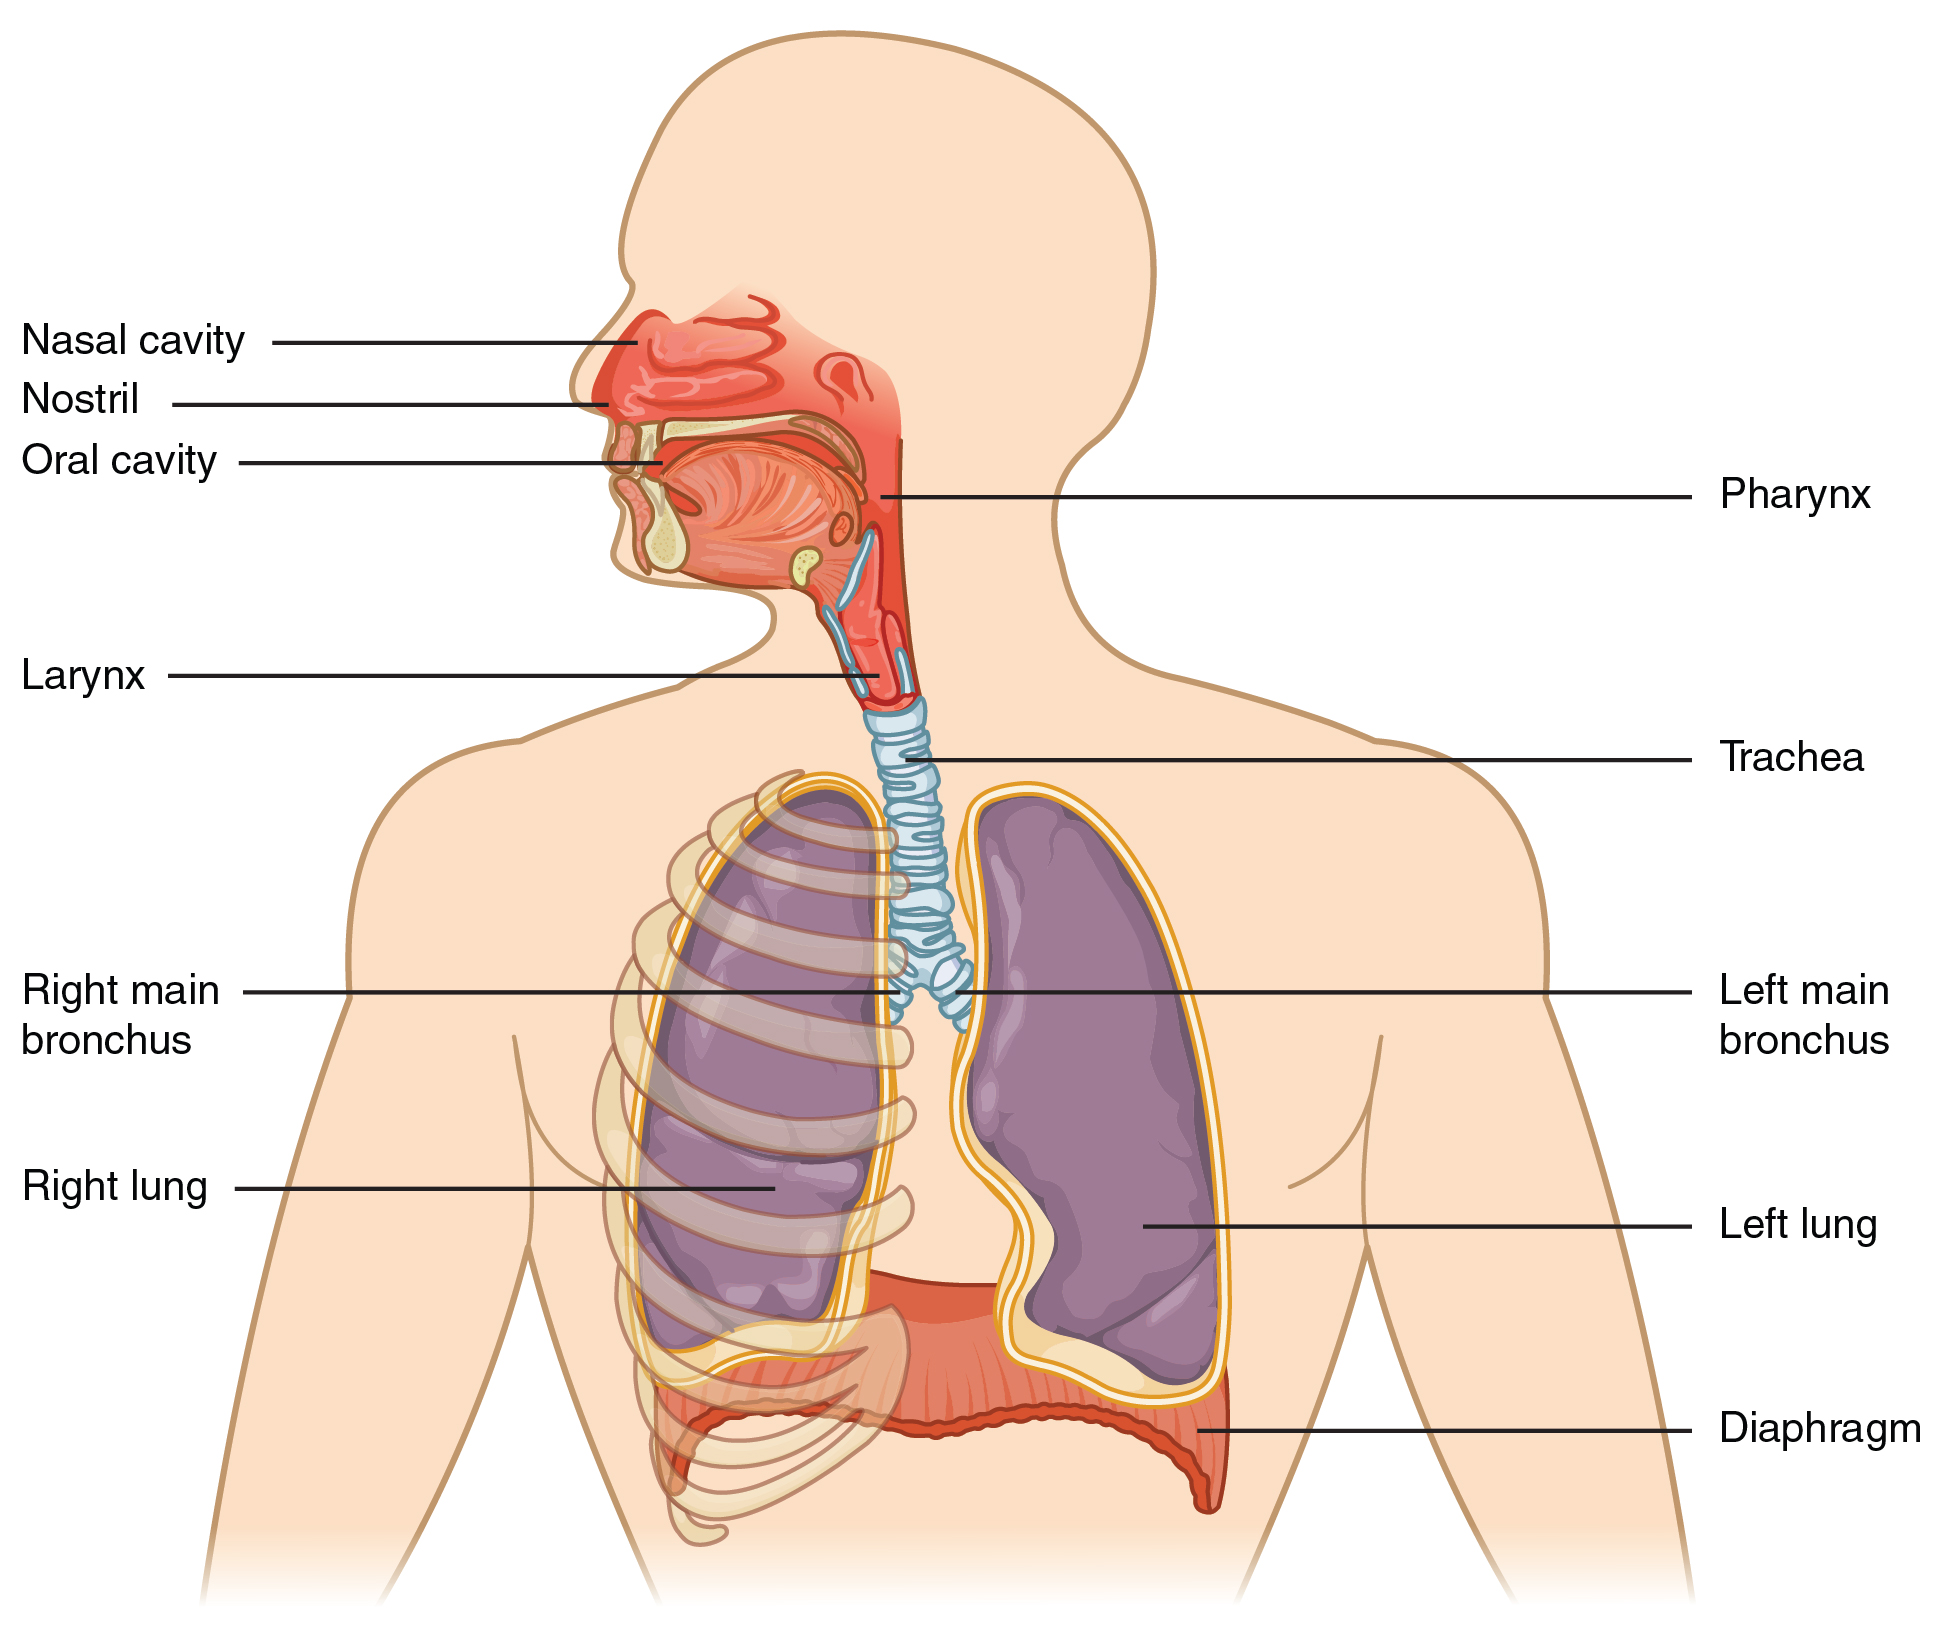
\includegraphics[width=0.5 \linewidth]{./figure/ventilation/airways.jpg}
    \caption{Major Airways and Anatomy of Ventilation \footnotesize{(OpenStax Anatomy, CCBYSA4.0)}}
    \label{fig:airways}
\end{figure}

\subsection{Anatomical Dead Space ($V_D_{ana}$)}

Any air that enters the airways is part of $V_e$, but it is not part of $V_A$ unless it reaches an alveoli. For example, at the end of an inspiration the air remaining in the upper airways (nasal passages, the back of the throat, trachea, bronchi, bronchioles) is part of $V_e$, but not part of $V_A$ (See Figure \ref{fig:airways_detailed}). 

\begin{figure}[!h]
    \centering
    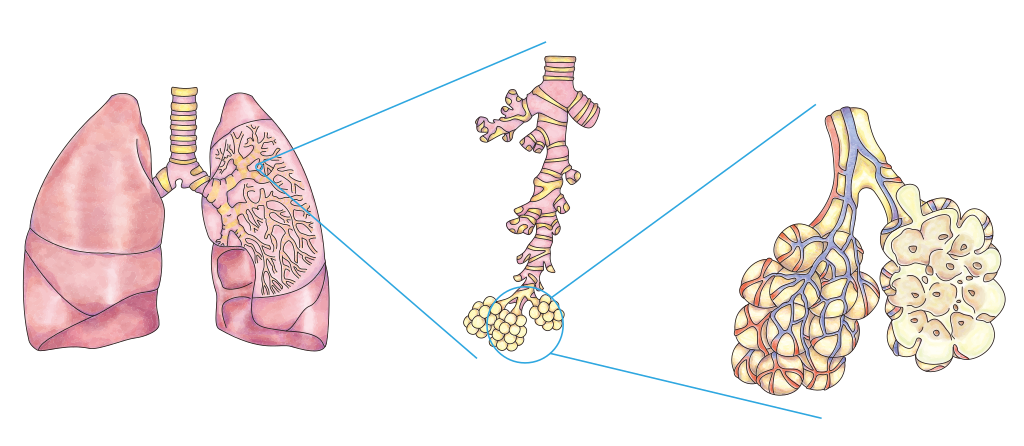
\includegraphics[width=1.0 \linewidth]{./figure/ventilation/airways_detailed.png}
    \caption{Detail of Airways from Trachea to Alveoli \footnotesize{(WikiMedia Commons, CCBYSA4.0)}}
    \label{fig:airways_detailed}
\end{figure}

Air in the airways that does not reach the alveoli (airway conduction zone) is anatomical dead space ($V_D_{ana}$). $V_D_{ana}$ is a considered fixed volume ($mL$) per breath. For example, if $V_D_{ana} = 100 mL$, and 400 $mL$ is inspired with tidal volume ($V_T$), then 300 ($mL$) reaches alveoli ($V_A$). 

The air that does reach the alveoli is alveolar ventilation ($V_A$), and is the ventilation minus the anatomical dead space ventilation:
\vspace{2mm}
\begin{equation}
    V_A (mL/min) = V_e (mL/min) - V_D_{ana} (mL/min)
    \label{eq:Va}
\end{equation}
\vspace{2mm}

\paragraph{Question:}

Does $V_A (mL/min)$ change if $V_e (mL/min)$ stays the same but is achieved with different volume ($mL$) per breath at different breathing frequencies (respiratory rates)? Answer this by figuring out the $V_A (mL/min)$ and $V_e (mL/min)$ if $V_D_{ana} = 100 mL$ per breath, when breathing 24 breaths per minute at 250 $mL/breath$; as compared to breathing 12 breathes per minutes at 500 $mL/breath$; as compared to breathing 6 breaths per minute at 1000 $mL/breath$. With each breathing pattern, $V_D_{ana} = 100 mL$ per breath since this is a fixed volume.

There are two approaches to this question. Both require using Equation \ref{Ve} ($V_e (mL/min) = V_t (mL) \times RR (bpm)$. The easiest approach is to substitute $V_e$ with $V_t (mL) \times RR (bpm)$ and adjust $V_t$ based on $V_D_{ana}$ since anatomical dead space occurs with each breath:

\begin{equation}
    V_A (mL/min) = (V_t (mL) - V_D_{ana}(mL)) \times RR (bpm)
\end{equation}

\subsection{Upper Airways}

The upper airways include the nasal passageways, the nasopharynx, and the pharynx. Down to the pharynx the oral passages are also an option for breathing, but mouth (oral) breathing is sub optimal. The nasopharynx passes into the oropharynx which passes into the hypopharynx (also called the laryngopharynx). At this point the epiglottis is the gatekeeper between the larynx (for air) and the esophagus (for food and drink).  The larynx is the beginning of the lower airways; it includes the vocal cords and then continues into the trachea. 

All airway passages down as far as the terminal bronchioles are lined with epithelial cells that include, in various locations, mucus production cells and cilia. Cilia are small cellular extensions that promote the movement of mucus across the membrane surface. Cilia move continually in a direction that moves mucus toward the pharynx. Mucus and cilia in the airways are combined as a defense mechanism referred to as mucociliary activity. Together they promote the trapping of particles in mucus (including pathogens) and moving the mucus for removal. Cilia movement in the lower airways (trachea and bronchi) is upward, whereas those in the upper airways is downward. Continual cilia movement moves the mucus toward the pharynx. The mucus and its trapped particles are then swallowed or coughed out of the body.

\subsubsection{Bronchopulmonary Hygiene \& Airway Clearance}
Mucocilary activity, along with regular deep breathing, is an important component of bronchopulmonary hygiene (BPH); while throat (pharynx) clearing, sneezing, coughing are airway clearance. Techniques to facilitate airway clearance are airway clearance techniques (ACT). BPH and ACT include several manual techniques within the physical therapy scope of practice.\footnotemark\footnotetext{Please don't tell me that "respiratory therapy" does this, of course they do. But that does not negate the fact that this is part of the PT scope of practice. If PTs did not do the things in their scope of practice that other professionals do, physical therapists would not do anything. Saying "respiratory therapy" does this - is like saying "massage therapists" do this about soft tissue mobilization; or that "chiropractors" do this about joint mobs/manipulations; or that "athletic trainers" or "OTs" do this about rehabilitation; or that "exercise physiologists" or "personal trainers" or "strength and conditioning specialists" do this about exercise prescriptions. Of course that is all true. Doing one thing is NOT what makes any of those professionals the professionals that they are, it is doing those things in context and the variety of things being done that makes each of these professions, including physical therapy. The PT uses BPH-ACT in in the plan of care for patients receiving PT, which will include many other interventions based on client needs.} Just as increasing tissue extensibility through manual techniques may facilitate the range of motion necessary to move during therapeutic exercise to then maintain tissue extensibility; improving ventilation and respiration through manual techniques may facilitate the respiration necessary to move during exercise to then maintain respiration.  

\subsubsection{Nasal Passageways} 
Nasal passageways are lined with epithelial cells rich in olfactory sensors (sense of smell) and goblet cells which are responsible for creating mucus. The passages include a set of turbinates that create turbulent flow of air through the passageways which is important for immunity, humidification, adding nitric oxide and the sense of smell. The turbulent flow of air encourages interaction between the air entering the the nasal passages and the cellular epithelial mucus membrane. Large particles (dust, pathogens, allergens) are very likely to become stuck in the mucus of the nasal passage membranes, serving an important immune and protective function. Interaction with the nasal passage membrane also humidifies the air (adds water) and adds nitric oxide (NO). NO enhances local defense mechanisms via direct inhibition of pathogen growth and stimulation of mucociliary activity. NO from the nose and sinuses is added to the air with every breath taken through the nose. NO reaches the alveoli in a more diluted form and enhances alveolar respiration by local vasodilation of pulmonary capillaries \cite{tornberg_nasal_2002, lundberg_nitric_2008}. For these, and many other reasons, nasal breathing is better for ventilation and respiration and promotes more efficient breathing. Nasal breathing tends to encourage and promote further nasal breathing. Mouth breathing tends to make nasal breathing more difficult. If someone that uses mouth breathing attempts to nasal breathe they may need to go through a transition period with intentional nasal breathing to help re-establish air movement through the nasal passageways. Mouth breathing has also been linked to sub-optimal changes to upper airways that ultimately make nose breathing more difficult which then promotes more mouth breathing. Mouth breathing is associated with snoring, sleep apnea and hyperventilation (over breathing) dysfunction \cite{gilbert_recognizing_2014}.

\subsubsection{Lower Airways}
The trachea is the airway that brings air to the many divisions that terminate in alveoli. The trachea is supported by cartilage rings that keep it open during wide fluctuations in thoracic pressures (coughing, sneezing, valsalva manuever\footnotemark\footnotetext{Valsalva manuever includes forced expiration against a closed epiglottis and the development of substantial intrathoracic, including intrapulmonary, positive pressure. It often occurs during straining for a bowel movement, or during lifting and is thought to provide stability support and counteract compression of the spine when combined with increased abdominal pressure. Risks include hernia, lung collapse (pneumothorax), and alterations to blood flow leading first to elevated and then dropped blood pressure.}). The trachea divides at the carina into two main bronchi (right and left) for the right and left lungs (respectively) (See Figure \ref{fig:lower_airways}). 

\begin{figure}[!h]
    \centering
    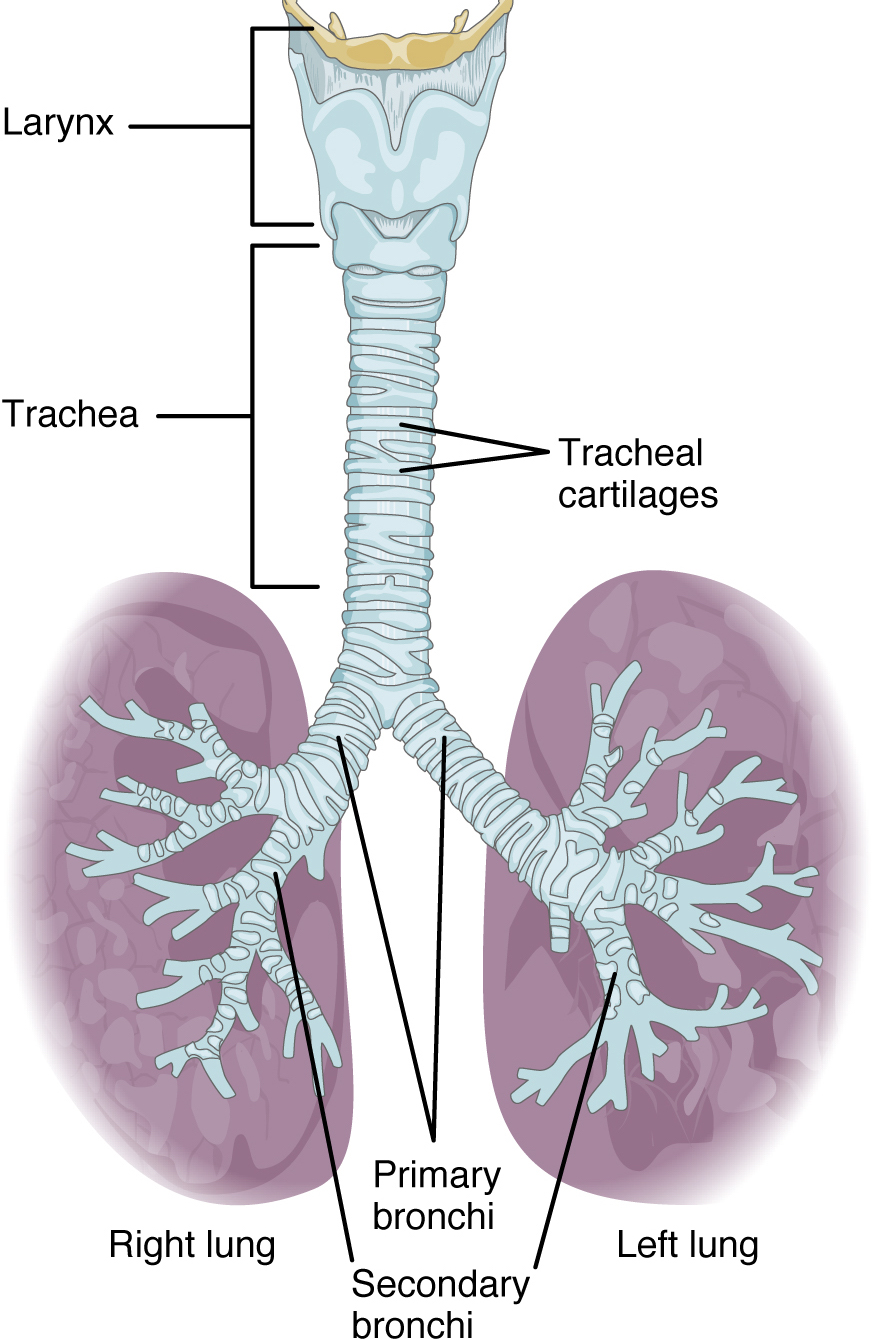
\includegraphics[width=0.4 \linewidth]{./figure/ventilation/lower_airways.jpg}
    \caption{Trachea and Main Bronchi Branches \footnotesize{(OpenStax, CCBYSA4.0)}}
    \label{fig:lower_airways}
\end{figure}

The main, and larger bronchi, also contain cartilage rings for support along with smooth muscle. Each bronchi splits into two branches for approximately 20-25 generations until ending with alveoli \cite{hall_guyton_2020}. The final branch of the bronchi is a terminal bronchiole and is sometimes referred to as the respiratory bronchiole (See Figure \ref{fig:alveoli}). The lower airways are also lined with epithelial cells that produce mucus and have cilia, and thus also have mucociliary activity that contributes to bronchopulmonary hygiene (BPH) and airway clearance. 

\begin{figure}[!h]
    \centering
    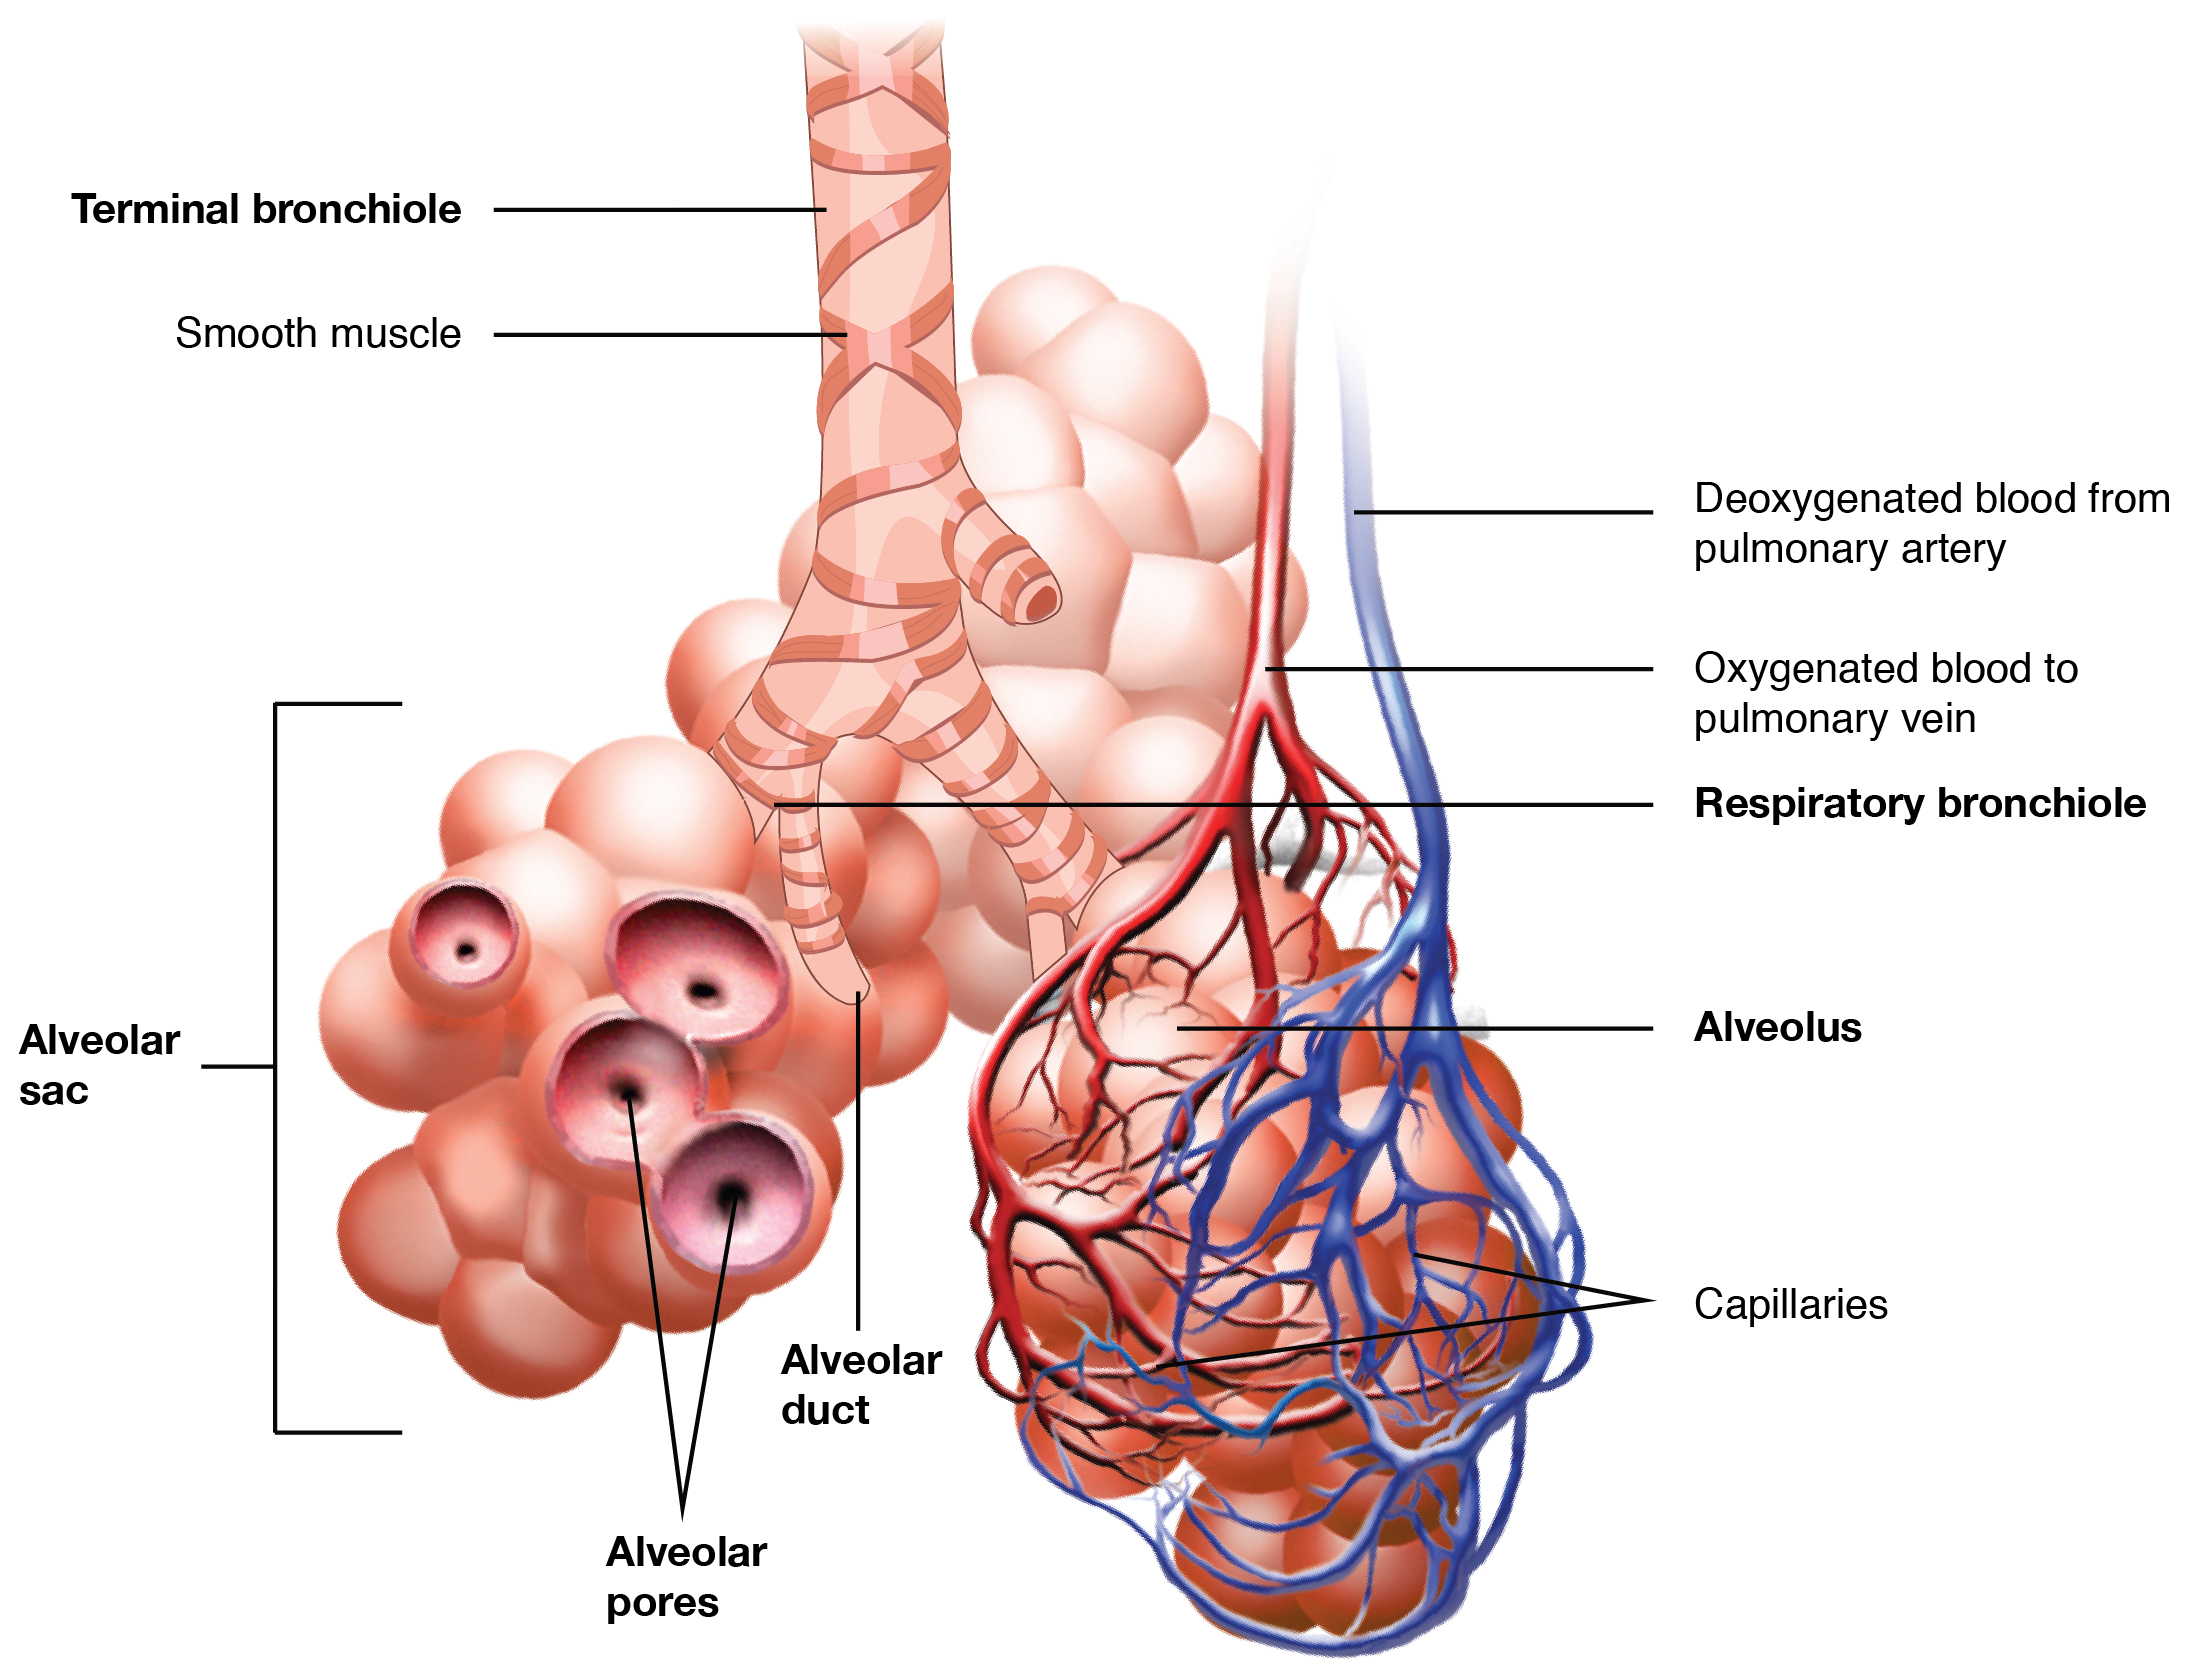
\includegraphics[width=0.5 \linewidth]{./figure/ventilation/alveoli.jpg}
    \caption{Terminal Bronchiole \& Alveoli \footnotesize{(OpenStax, CCBYSA4.0)}}
    \label{fig:alveoli}
\end{figure}


Similar to the artery to arteriole, each branch of the the bronchi to bronchiole gets progressively smaller, while the sum of space gets larger; and the influence of smooth muscle on the radius gets more important. For example, the main bronchi is larger than any single branch, but the branches, summed together, offer far more space than the main bronchi. As the branches get smaller with each generation of splitting the walls get thinner and the influence of smooth muscle on the walls gets more influential. Most bronchodilation and bronchoconstriction occurs in the smaller bronchioles than in the larger bronchi.

Under normal conditions resistance to air flow is highest in the larger bronchi because there are relatively few bronchi compared to bronchioles. But with various pulmonary conditions the smaller bronchioles play a greater role in determining air flow resistance for two reasons. First, they are easily occluded because of their small size. Second, they are easily constricted because they have a greater proportion of smooth muscle fibers in their walls in relation to their radius and they do not have supportive cartilage rings.

The factors impacting air flow, like blood flow, through a cylinder such as an airway (or blood vessel) can be considered with Pouiselle's Law:
\vspace{3mm}
\begin{equation}
    Flow = \frac{\pi \times \Delta P \times r^4}{\eta \times L}
\end{equation}
\vspace{3mm}
And similar to blood flow, the resistance to airflow is largely determined, and manipulated, by changes to the radius through bronchodilation and bronchoconstriction.


\paragraph{Bronchodilation \& bronchoconstriction} are regulated by sympathetic nervous system innervation and endocrine function (circulating epinephrine and norepinephrine). Control of the bronchioles by sympathetic nerve fibers is relatively weak because few nerve fibers penetrate deeply and reach the bronchioles. However, all bronchi and bronchioles are exposed to circulating norepinephrine and epinephrine released from the adrenal medulla. These hormones, and in particular epinephrine because of its greater stimulation of $\beta$-adrenergic receptors, dilate bronchi and bronchioles. A few parasympathetic nerve fibers, from the vagus nerve, reach the bronchi and bronchioles. These nerves secrete acetylcholine, which constrict the bronchi and bronchioles. 
Conditions that create bronchoconstriction, such as asthma, are therefore commonly treated with $\beta$-adrenergic agonist inhalers (inhaled medication), sometimes in combination with cholinergic antagonist inhalers. A side effect of $\beta$-adrenergic agonist inhalers is anxiety and rapid heart rate. This side effect would be much more pronounced if the $\beta$-adrenergic agonist was taken orally and not with an inhaler because of its impact on the heart.

\section{Volumes \& Capacities}

Ventilatory volumes and capacities are depicted in Figure \ref{fig:ventilation_volumes}. Capacities are combinations of volumes.

\begin{figure}[!h]
    \centering
    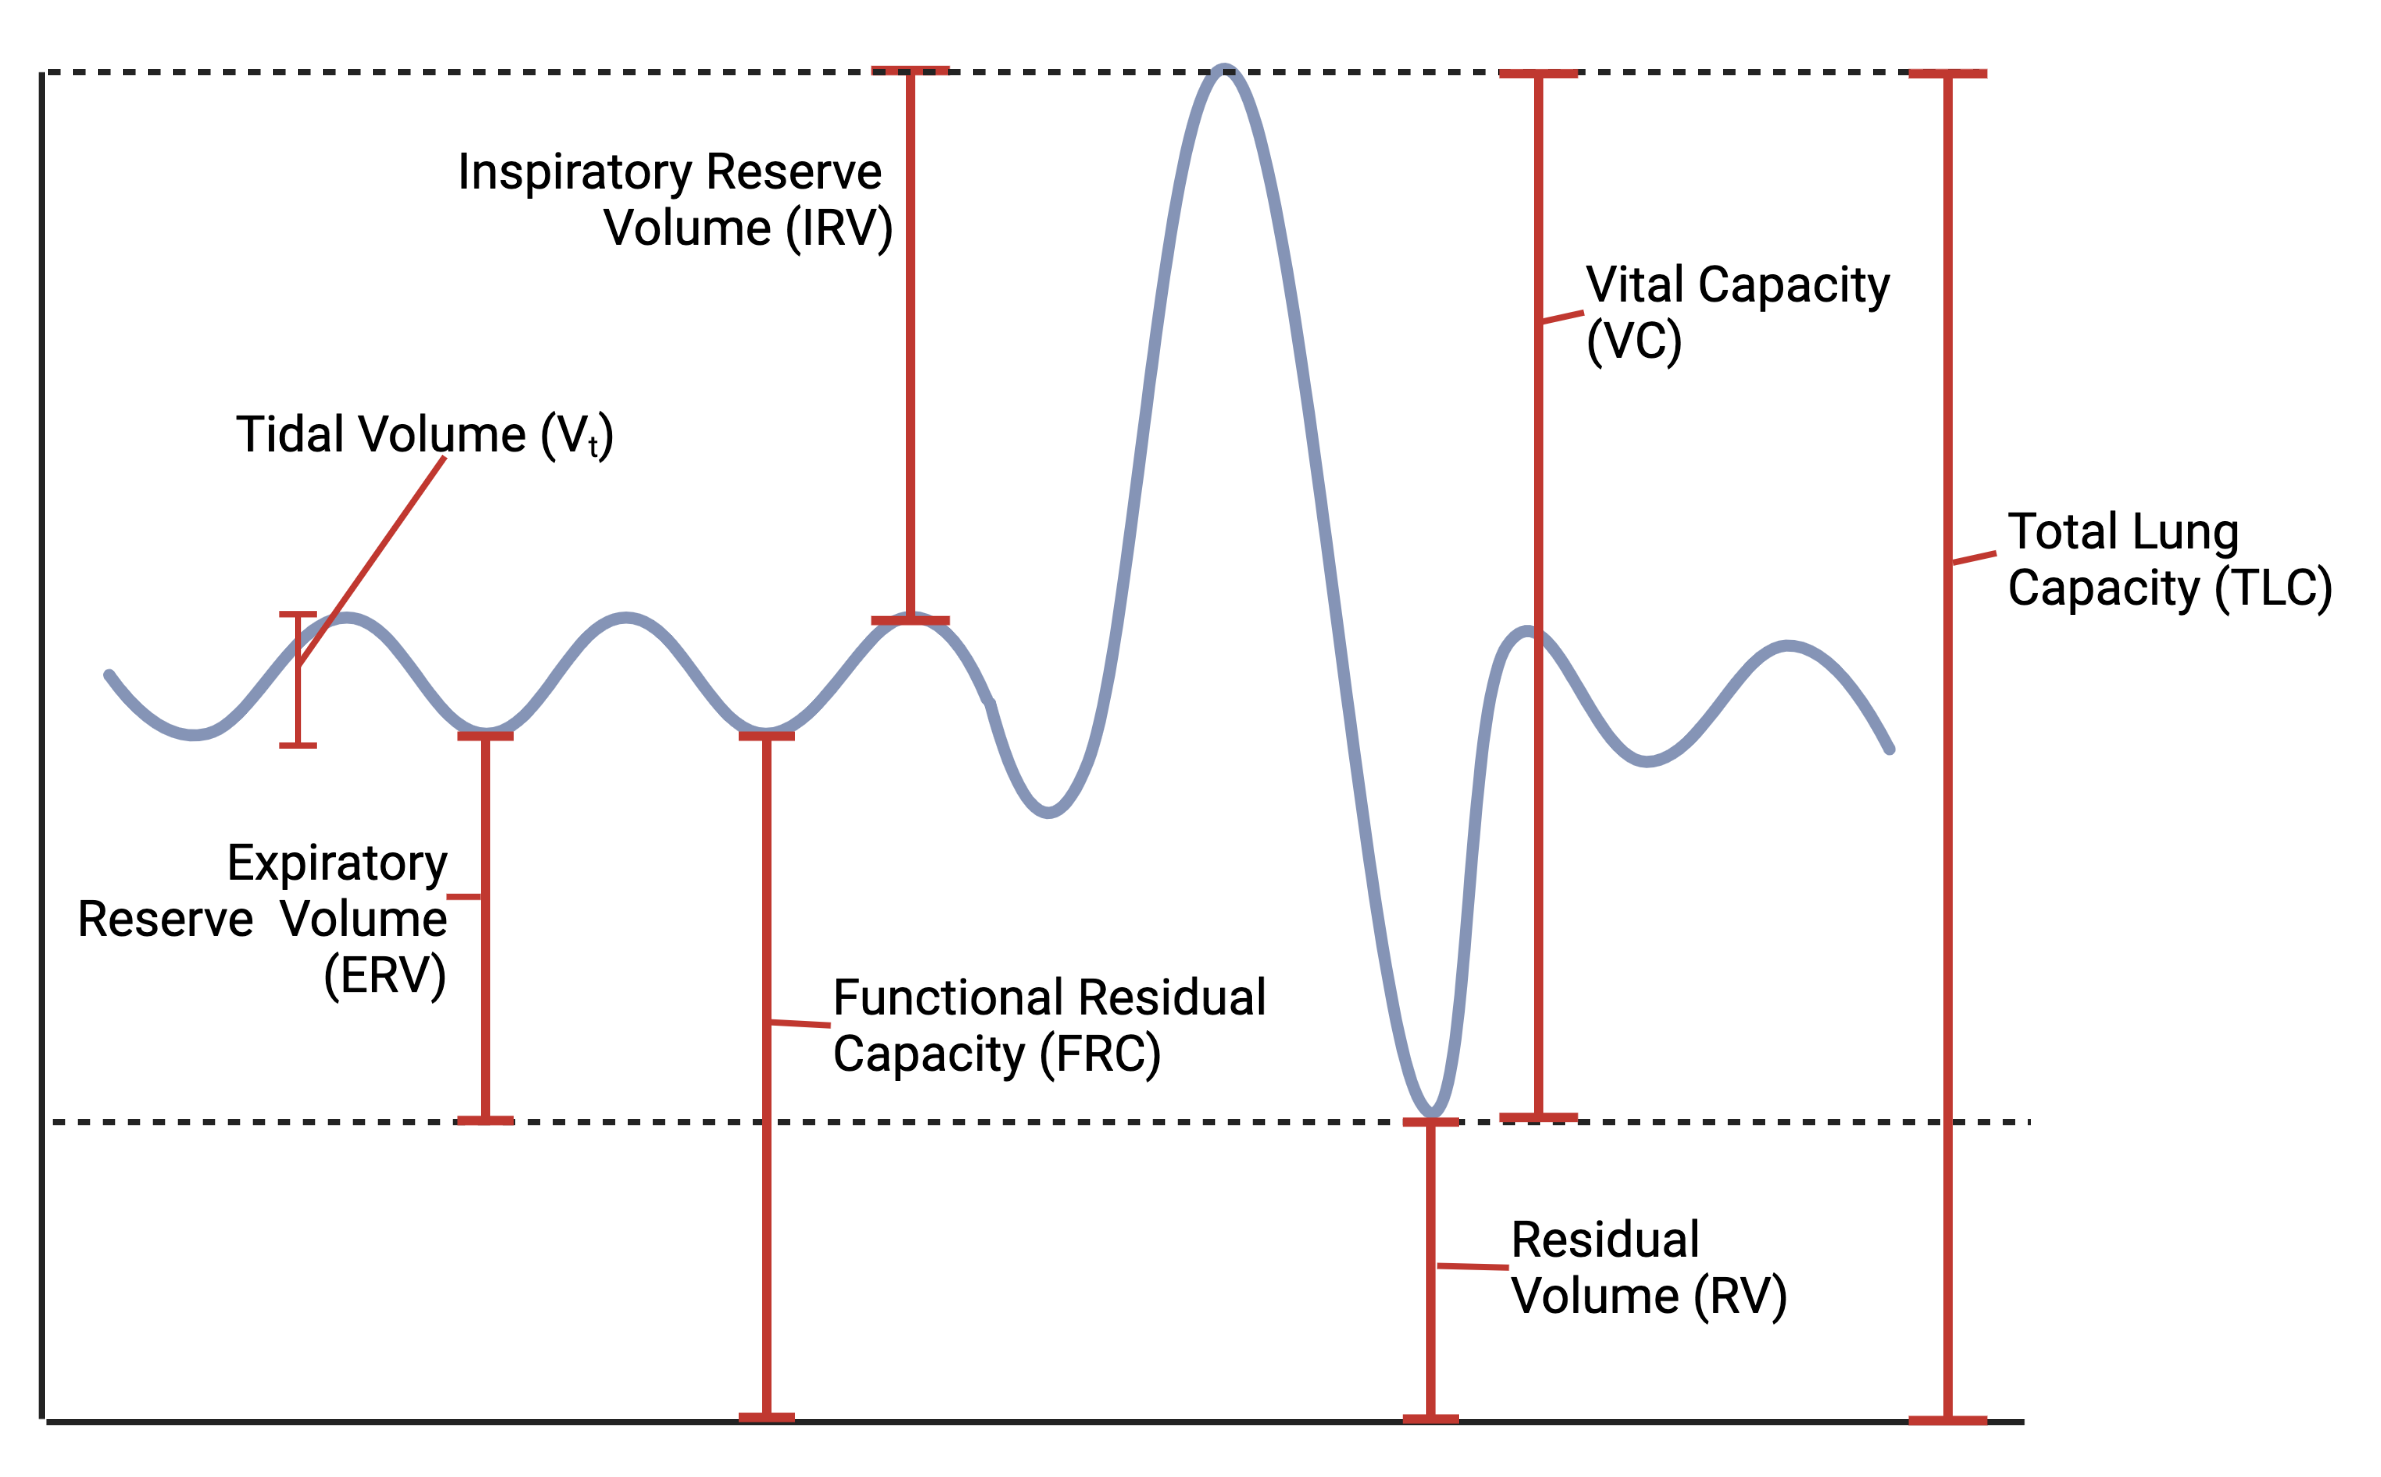
\includegraphics[width=0.75 \linewidth]{./figure/ventilation/ventilation_volumes.png}
    \caption{Ventilatory Volumes \& Capacities}
    \label{fig:ventilation_volumes}
\end{figure}

\begin{itemize}
    \item Tidal Volume ($V_t$): Volume of breathing. $V_t$ varies in order to change ventilation $V_e$, for the purpose of changing $V_A$ to meet the needs of alveolar respiration as it maintains $Pa_CO_2$ and $P_aO_2$; or adjusts $Pa_CO_2$ as part of acid base balance regulation.
    \item Inspiratory Reserve Volume ($IRV$) is the volume that can be inhaled after a normal $V_t$ inspiration
    \item Expiratory Reserve Volume ($ERV$) is the volume that can be exhaled after the end of a normal $V_t$ expiration
    \item Residual Volume ($RV$) is the volume that cannot be exhaled
    \item Vital Capacity ($VC$) is $V_t + ERV + IRV$, it is the largest volume that can be breathed in after a complete exhalation, or out after a complete inspiration
    \item Functional Residual Capacity ($FRC$) is $ERV + RV$, it is the volume of air remaining in the lungs after a normal expiration
    \item Total Lung Capacity ($TLC$) is $IRV + V_t + ERV + RV$, it total capacity for air in the lungs
\end{itemize}

\paragraph{The Musculoskeletal Side of Ventilation:} Volumes \& capacities are measures of the amount of air that can be ventilated (or that cannot be ventilated in the case of $RV$ which cannot be expired). They are helpful for understanding the functional capabilities of the lungs and describe changes to the lung in various states of disease. For example, with the obstructive pulmonary diseases the $RV$ tends to be higher, which reduces $VC$ (and all other values, except $FRC$). The volumes \& capacities also represent a functional measure of the thoracic cavity musculoskeletal range of motion (chest wall mobility) which includes the diaphragm, muscles of the ribs (intercostal muscles), the mobility of the ribs, and the posture of the spine. For example, in situations with diaphragm weakness, reductions in $VC$ are directly related to an inability of the diaphragm to fully descend against the combined resistance of pulmonary elasticity, thoracic muscles and joints, and abdominal contents. In patients with many different neurological conditions there is involvement of ventilatory muscles or spinal posture which greatly influence the ventilatory volume \& capacities that further limit activities and result in pulmonary conditions such as pneumonia.

\paragraph{Volumes \& Capacities as range of motion (ROM) - Chest Wall Excursion (CWE):} Occasionally the volumes and capacities are utilized as an indication of the chest wall range of motion (ROM), which is referred to as chest wall excursion (CWE). During testing of the strength of inspiratory muscles patients are asked to expire all their air prior to the test because it is best to test those muscles when they are stretched. Those muscles are stretched when they are in the CWE associated with and at the ROM of, $RV$. When doing a forced expiration, or when training someone to improve their cough, they are asked to take in a full breath, they breathe in until they are at the CWE associated with $TLC$. CWE can also be measured as a circumference, but not without limitations. One limitation is that the CWE with a tape measure is measuring circumference in one plane (even if it is an oblique plane, it is only one plane). Whereas the change in thoracic cavity size occurs in all three planes (all three dimensions). If CWE is measured with a tape measure, it is usually recommended that it is measured in more than one place (for example, above, at and below the xiphoid process). CWE is also assessed qualitatively simply by placing the hands on various locations of the chest wall and assessing the symmetry, amount and quality of movement.

\paragraph{Homeostatic Regulation with Volitional Control:} Ventilation is certainly part of an intricate set of homeostatic regulation mechanisms. Yet it is also under volitional control. The volitional control allows speech (vocalization), and it also allows the opportunity to use breathing to manipulate (hack) homeostatic systems that cannot otherwise be regulated directly (e.g. the use of deep breathing to increase parasympathetic nervous activity and lower heart rate). Physical therapists contribute uniquely to problems related to breathing and ventilation because of how much these processes rely on the neuromuscular mechanics of the breathing muscles. Like posture, gait and many movements, the breathing muscles and patterns of ventilation are mostly automatic yet are able to be voluntarily controlled, and therefore manipulated, adapted and trained. Emotional states are related to the autonomic nervous system (bi-directionally), and the autonomic nervous system (ANS) is related to breathing (bi-directionally). The bi-directional connection between ANS and breathing can be used to influence ANS by voluntarily altering breathing (See Figure \ref{fig:homeostatic_feedback}). The downside of this is that breathing dysfunction, even when not due to pulmonary disease but rather caused by altered breathing coordination (mechanics) or patterns, can result in altered emotions. Questionnaires to assess whether breathing coordination (mechanics)(including too much mouth breathing) or patterns may be impacting health include a host of signs and symptoms related to the ANS \cite{gilbert_recognizing_2014}.

\begin{figure}[]
    \centering
    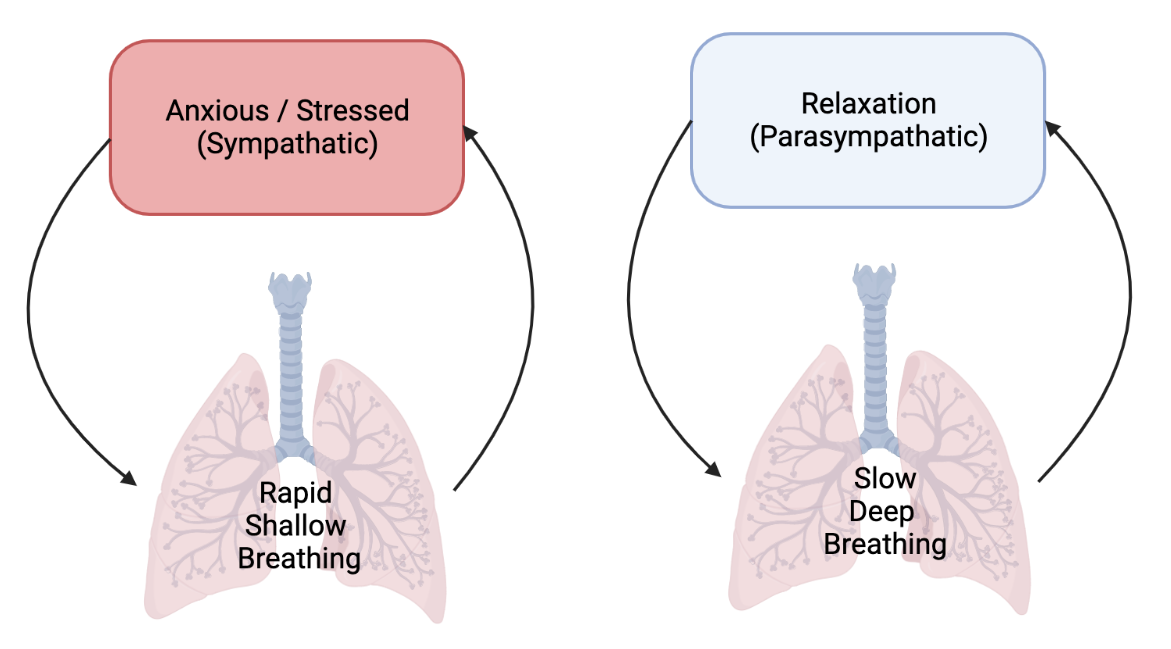
\includegraphics[width=0.65\linewidth]{./figure/ventilation/homeostatic_feedback.png}
    \caption{Bi-Directional Homeostatic Feedback Between Emotion and Breathing}
    \label{fig:homeostatic_feedback}
\end{figure}

\section{Mechanics: The Ventilatory Pump}

The ventilatory pump creates pressure for ventilation with the musculoskeletal system of the thorax (chest wall), including the diaphragm as the floor of the thoracic cavity (and roof of the abdominal cavity, See Figure \ref{fig:diaphragm_lateral}). The diaphragm is positioned to contribute to the variation of pressures between the thoracic and abdominal cavities which makes it uniquely involved in breathing as well as the coordination of breathing with other aspects of dynamic core stability. 

\begin{figure}[!h]
    \centering
    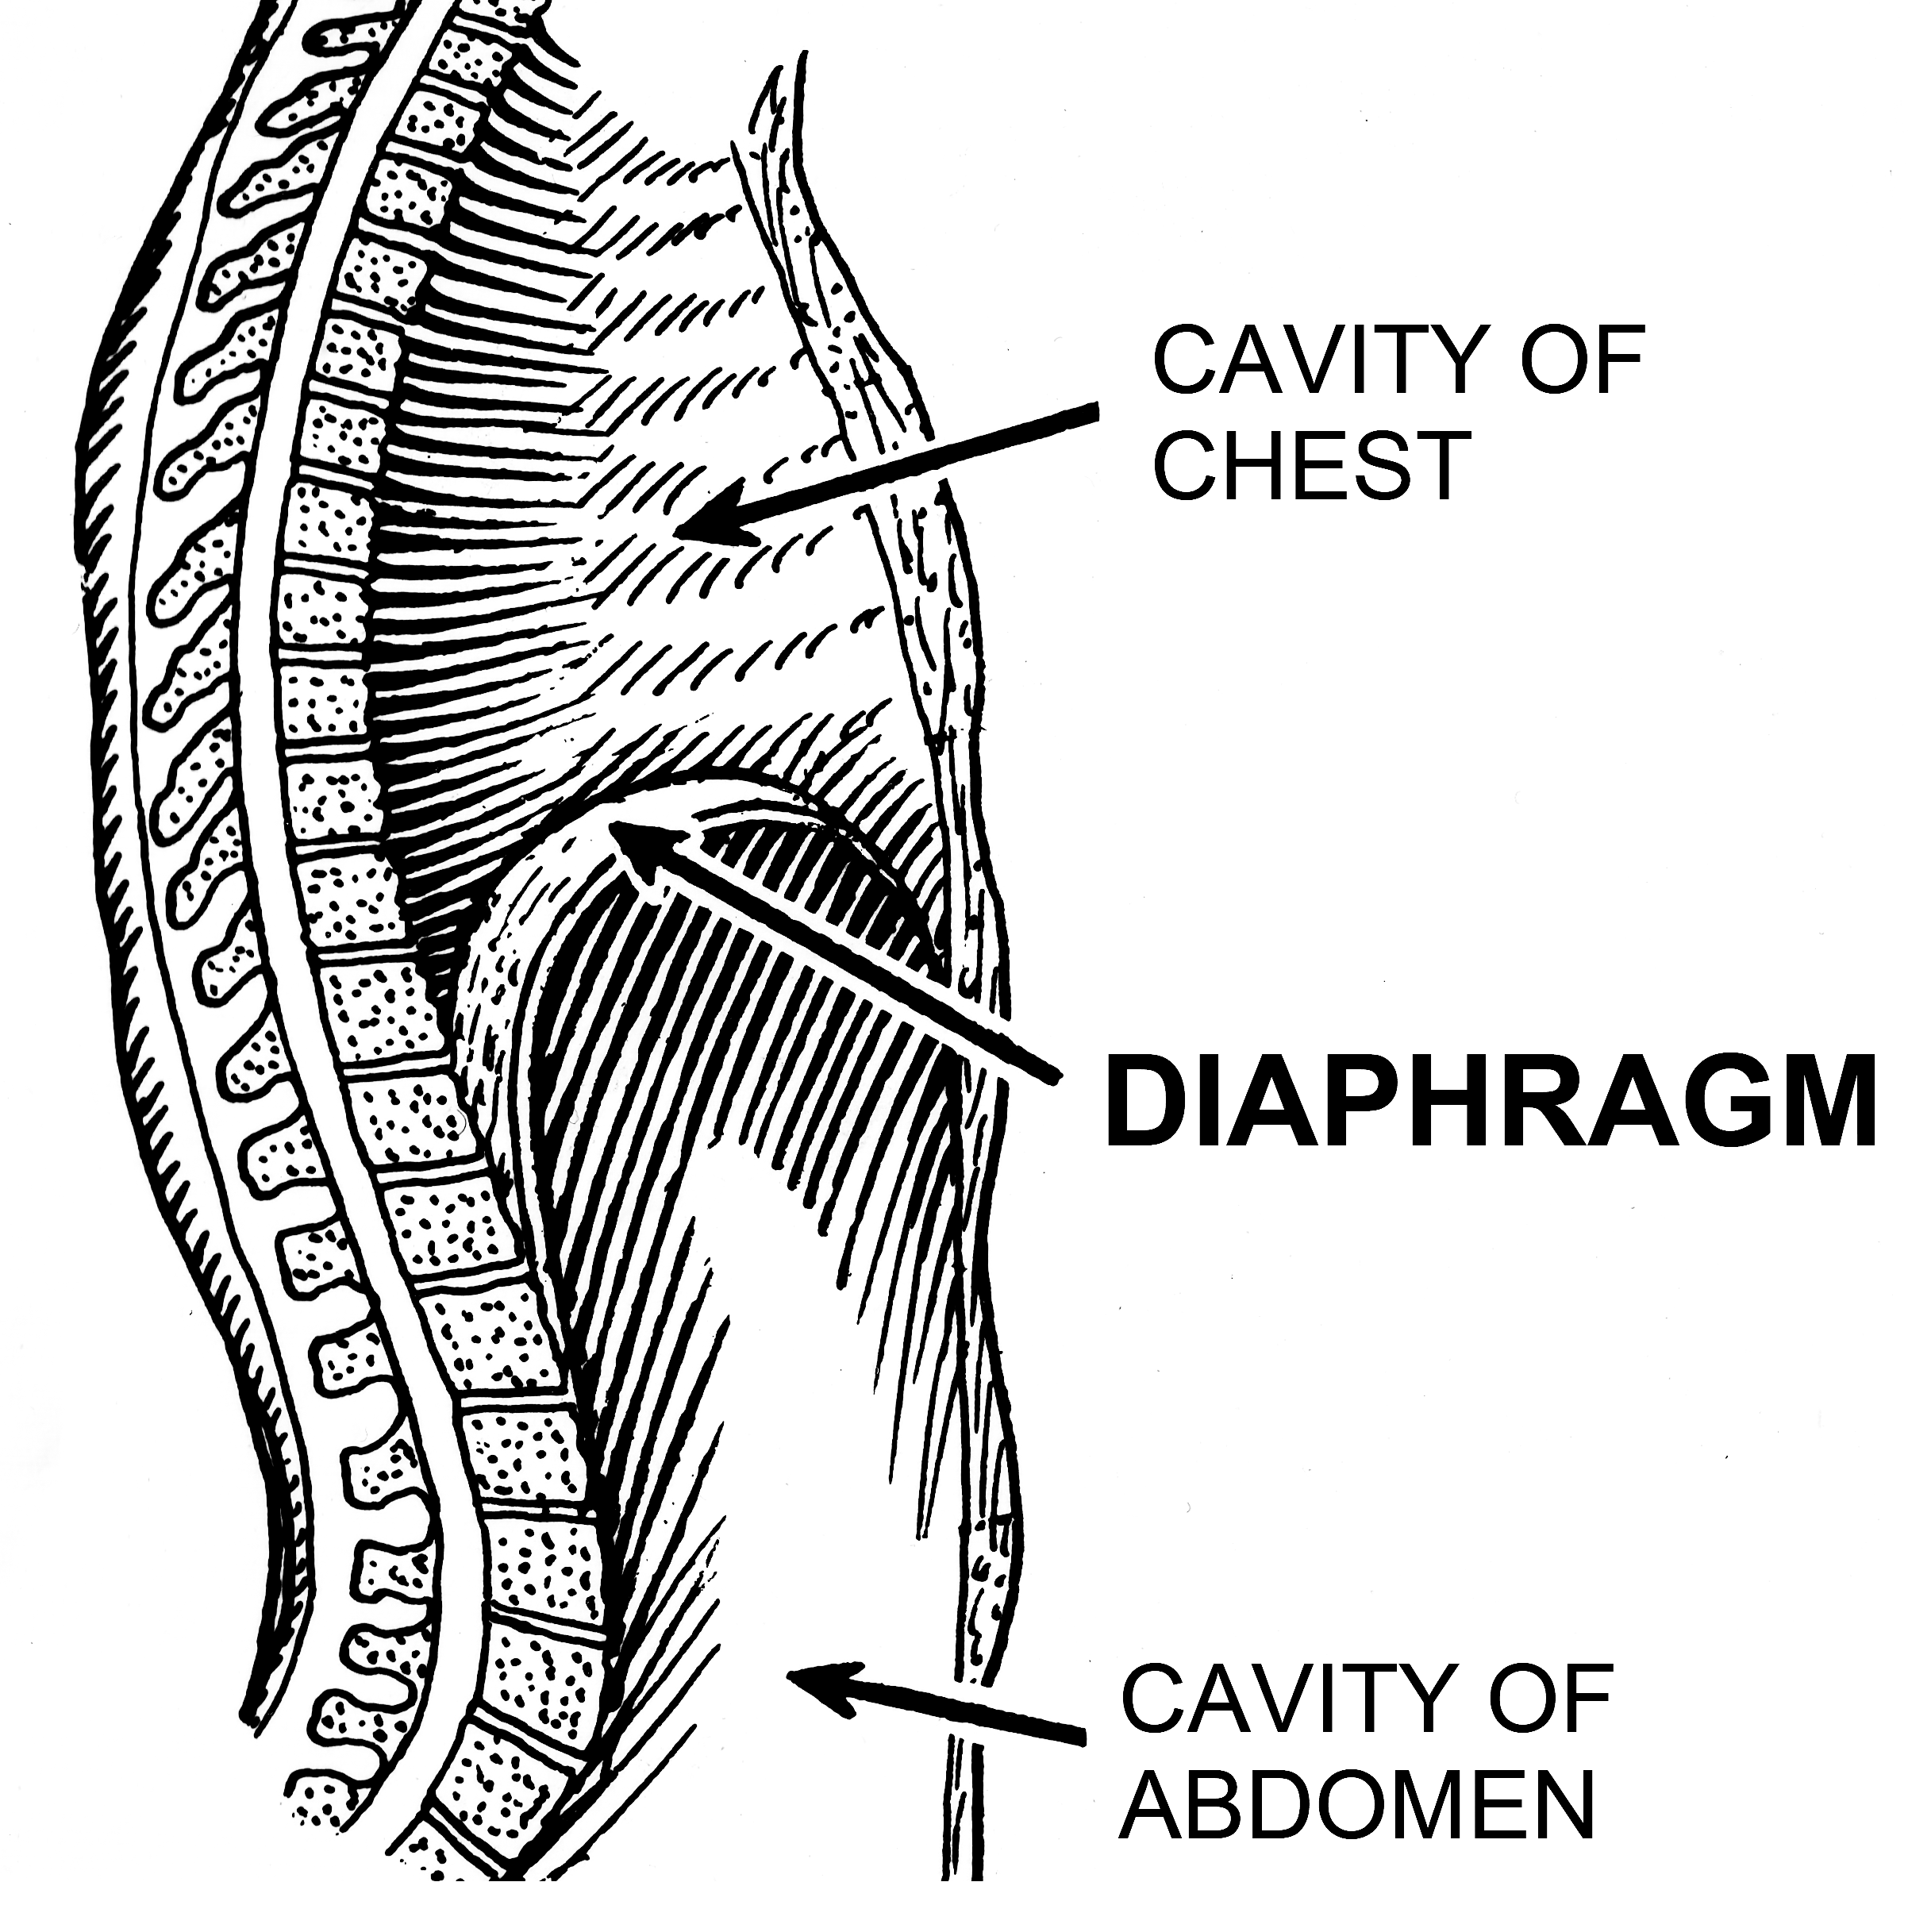
\includegraphics[width=0.35 \linewidth]{./figure/ventilation/diaphragm_lateral.png}
    \caption{Lateral View of the diaphragm dome and the separation between the thoracic and abdominal cavity \footnotesize{(CCBYSA4.0, WikiMedia Commons)}}
    \label{fig:diaphragm_lateral}
\end{figure}

\subsection{Inspiration: A Negative Pressure Pump} 
To breathe air into the lungs the ventilatory pump creates negative pressure. For breathing, the terms negative and positive pressure are always being compared with the atmospheric pressure. Negative pressure means less than atmospheric pressure; and positive pressure means greater than atmospheric pressure. When the ventilatory pump generates negative pressure it pulls air into the lungs. It does this by expanding the volume of the thoracic cavity, which lowers the pressure below the atmospheric pressure to establish the necessary pressure gradient for air flow. Based on the familiar equation: $Flow = (P_1 - P_2) / R$; the flow is directly proportional to the pressure gradient created, and inversely proportional to the resistance (and the resistance is largely dependent on the radius of the airways). 

\subsection{Expiration: A Positive Pressure Pump} For breathing air out of the lungs the ventilatory pump is a positive pressure pump. Positive pressure is generated by reducing the volume of the thoracic cavity, which increases the pressure above the atmospheric pressure to establish the necessary pressure gradient for air flow. Air flow is still directly proportional to the pressure gradient, and inversely proportional to resistance. Resistance is still largely dependent on the radius of the airways. 

One difference with expiration is that the positive pressure, combined with the fact that during expiration the lungs and airways are getting smaller, it is much more likely that resistance to expiratory flow will impact exhalation (than resistance to inspiratory flow will impact inhalation). The practical implications are that with any condition that impacts airway radius, such as asthma, emphysema and chronic bronchitis, the functional impact is on expiratory flow rates more than inspiratory flow rates. When a limitation is made on expiratory flow rates the term utilized to describe the pattern is obstructive. 

Forced expiratory activities - such as airway clearance with sneezing or coughing - requires a rapid increase in positive thoracic pressure. The difference between a sneeze (besides being typically through the nose) and a cough is closure of the epiglottis to allow for a larger build up of positive pressure in the thoracic cavity and a sudden release of that pressure when the epiglottis opens.  

\subsection{Pressure Equilibration} 
Airflow through airways is rapid enough that equilibration can occur at any thoracic cavity volume. Once equilibration occurs, airflow stops. This means that at any thoracic cavity volume, other than $TLC$ or $RV$, changes in volume can cause either inspiration or expiration depending on how the changes in volume change the pressure. At this point it's helpful to remind readers of the Ideal Gas Law (in fact, this needs to be introduced earlier to avoid confusion in future versions....). 

The common form of the Ideal Gas Law is: 

\begin{equation}
    PV = nRT
    \label{ideal_gas}
\end{equation}

Where, $P$ is pressure; $V$ is volume, $n$ is the number of moles in the gas (the amount of gas), $R$ is a gas constant, and $T$ is the temperature in Kelvin. For our purposes we can simplify by removing $R$ and $T$ (although there are slight changes during ventilation from the temperature of atmospheric air and the warmed air at body temperature, these are relatively small on the Kelvin scale, and since we are not actually calculating just considering relationships, we'll be fine).

A simplified version of the Ideal Gas Law, that solves for $P$ is:

\begin{equation}
    P = \frac{n}{V}
\end{equation}

An increase in the thoracic cavity $V$ will reduce the $P$. The reduced $P$ results in air flow into the lungs through airways until the amount of air in the lungs $n$ raises $P$ until it equals the atmospheric pressure and air stops flowing into the lungs. At that point, if thoracic cavity $V$ can be increased more then $P$ will drop and more air will flow into the lungs until $n$ increases to the point that $P$ in the lungs equilibrates with the atmospheric pressure. 
The same process can be considered for exhalation. A reduction in thoracic cavity $V$ increases the $P$, air flows out of the lungs until $n$ is reduced until $P$ equals the atmospheric pressure. 

\paragraph{Breathing in, Breathing out} is a cyclic variation in the difference between the thoracic (pulmonary) $P$ and the atmospheric pressure, brought on by the cyclic variation in the thoracic (pulmonary) $V$, which is equilibrated by the movement of air into (increase $n$) and out of (decrease $n$) the lungs.

\subsection{$FRC$: The Resting Position}

When considering the mechanics of the ventilatory pump during breathing it is useful to understand the conditions surrounding the functional residual capacity ($FRC$). $FRC$ is the resting position (volume) of the thoracic cavity, and therefore the amount of air in the lungs at this position equals the $FRC$. (That's a nice, intentionally, circular explanation.) 
$FRC$ is the $V$ of the thoracic cavity when there is no active tension being developed by the breathing muscles. The $V$ of the thoracic cavity can still change based on body position, but it is not changing due to active tension of breathing muscles (either inspiratory or expiratory muscles). If you "stop breathing" - and there is no airflow - you are at $FRC$. If you do this in standing and then sit down there may be slightly less $V$ at $FRC$. If you are seated upright and slouch or lean forward then you reduce the $V$ and $FRC$. The $FRC$ is the $V$ in the lungs when there is no active attempt to breath, but it is positionally (supine, prone, sitting, standing) and posturally (spine neutral, flexed, extended) dependent.

\paragraph{$FRC$ is the balance point} between an inward elastic recoil force of the lung tissue, and an outward elastic recoil force of the musculoskeletal thoracic cavity and is influenced by other forces such as gravity (and the impact that gravity has on the thoracic cavity) (See Figure \ref{fig:frc}). If the lungs were removed from the body (or detached due to a loss in negative pleural pressure), they would be smaller (less $V$) than at the $FRC$. Without the influence of the lungs, the thoracic cavity would be larger (more $V$) than at the $FRC$. 



\begin{figure}[!h]
    \centering
    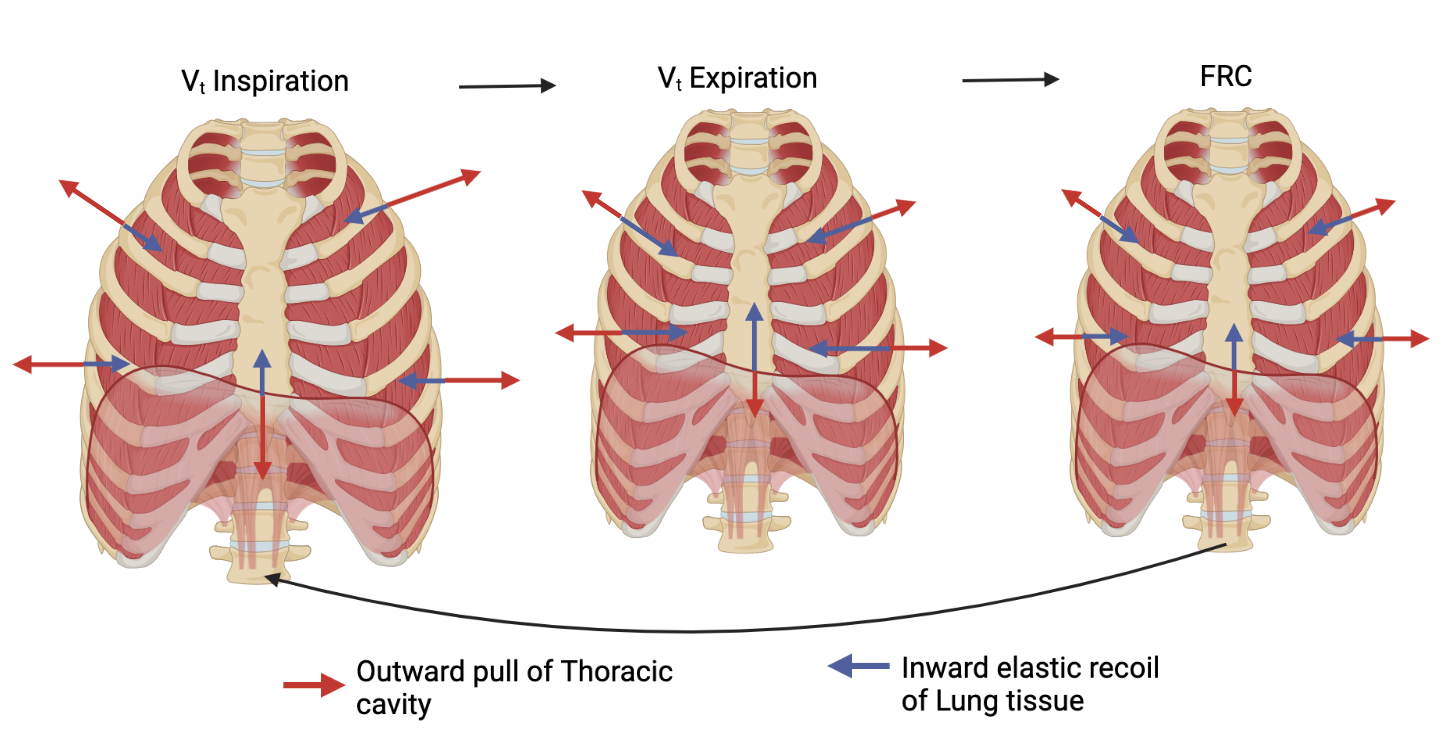
\includegraphics[width = 1.0 \linewidth]{./figure/ventilation/frc.png}
    \caption{Inward Elastic Recoil of Lung Tissue, Outward Pull of Thoracic Cavity. FRC occurs at the end of passive expiration at the balance point of these forces. \footnotesize{(Created with BioRender.com)}  }
    \label{fig:frc}
\end{figure}

The balance of forces point of $FRC$ has a large influence on breathing patterns because it has a large influence on optimal breathing volumes. During resting tidal volume ($V_t$) breathing each expiration ends at $FRC$ and therefore is a passive process. Another way to say this is that a resting $V_t$ expiration ends at $FRC$ so that it can be a passive process. Inspiration requires muscles of inspiration to expand the thoracic cavity $V$, working against the passive recoil force of the lung tissue. But then the passive recoil force of the lung returns the $V$ to $FRC$ which promotes expiration. Therefore, with resting $V_t$ breathing only the muscles of inspiration must be utilized. 

During resting $V_t$ breathing, initial increases in thoracic cavity $V$ are easier to perform because the thoracic cavity is naturally larger than at $FRC$. However, with increases in thoracic cavity $V$ both the lungs and the thoracic cavity create a passive elastic force that the muscles of inspiration must oppose for continued inspiration. This is one of the reasons that during exercise, breathing patterns typically increase $V_t$ by using more of the $ERV$ as compared to the $IRV$.

Forceful expiration requires a larger and more rapid change in $P$, which requires a larger and more rapid change in $V$, which requires active tension in the muscles of expiration. Increasing the rate of breathing $RR$ alone, or along with an increase in $V_t$, requires active tension of the expiratory muscles so that it occurs more completely (volumes less than $FRC$), and more quickly. 

\subsection{Muscles of Inspiration: Increase Thoracic Cavity Volume}

\subsubsection{Diaphragm}

The diaphragm is a membranous muscle and is the most important inspiratory muscle, with motor innervation solely from the phrenic nerves (C3-C5). The diaphragm is extremely active. Muscle fibres within the diaphragm can reduce their length by up to 40\% between residual volume and total lung capacity and spend 35\% of each day in an active tension state \cite{lumb_nunns_2020}. The origins of the crural part of the diaphragm are the lumbar vertebrae and the arcuate ligaments, while the costal parts arise from the lower ribs and sternum. Both parts are inserted into the central tendon (See Figure \ref{fig:diaphragm_inferior}). 

\begin{figure}
    \centering
    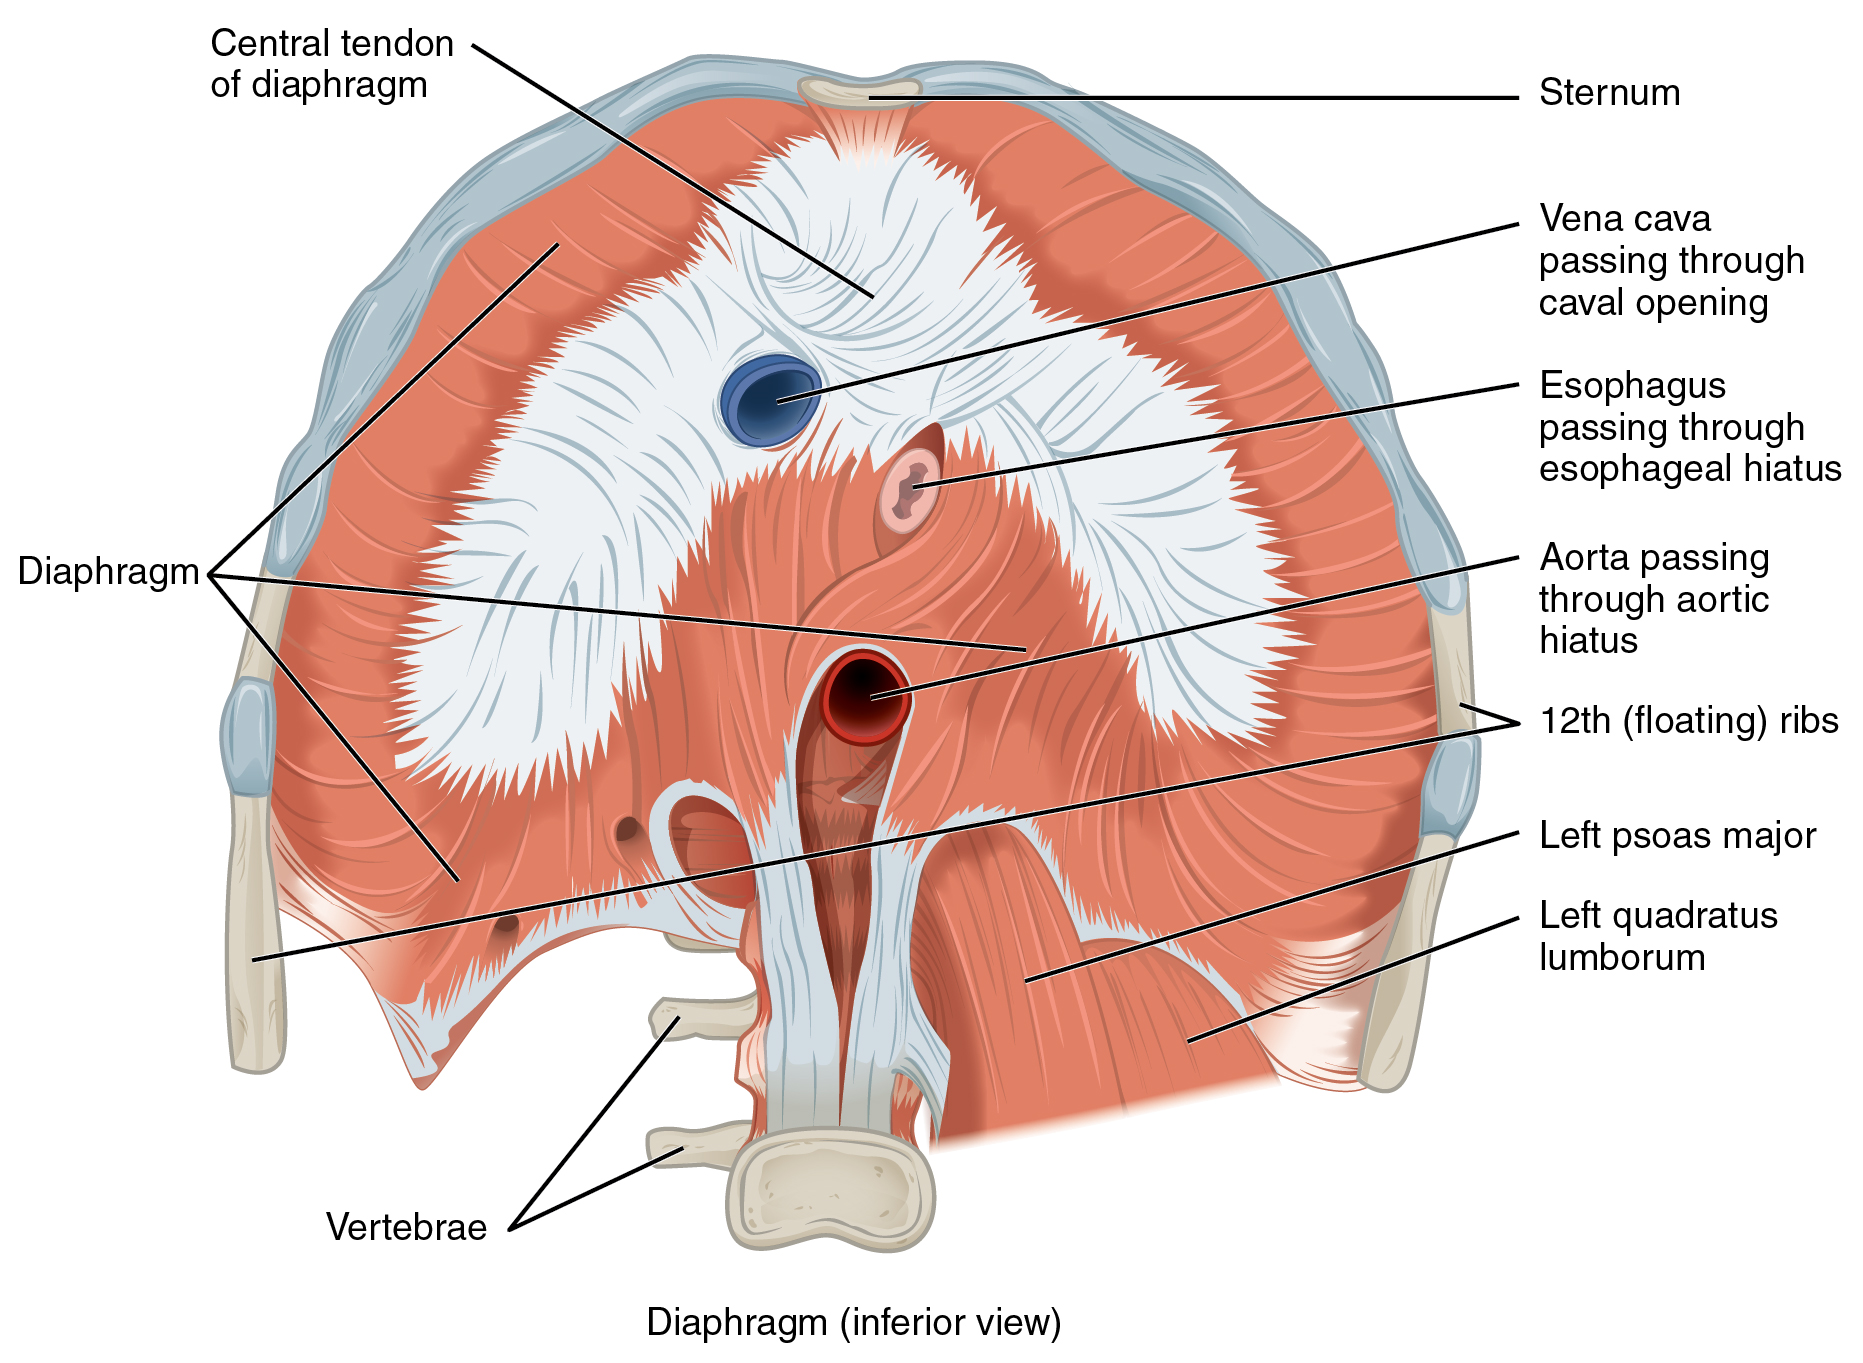
\includegraphics[width=0.75 \linewidth]{./figure/ventilation/diaphragm_inferior.jpg}
    \caption{Inferior View of Diaphragm Attachments \footnotesize{(OpenStax, CCBYSA4.0)}}
    \label{fig:diaphragm_inferior}
\end{figure}

Under normal circumstances, a zone of apposition exists around the outside of the diaphragm where it is in direct contact with the inside of the rib cage, with no lung in between. The parietal pleura continues to allow movement of the diaphragm. When at the upright $FRC$ approximately 55\% of the diaphragm surface area is in the zone of apposition (See Figure \ref{fig:diaphragm}).

There are three actions that the diaphragm creates to increase thoracic cavity $V$ and these three actions are combined during breathing. Diaphragm mechanics, and these three actions, can be considered with the analogy to a piston in a cylinder. With the diaphragm being the piston, and the thoracic cavity being the cylinder. A graphic of these three diaphragm actions is depicted in Figure \ref{fig:diaphragm}. 

\begin{enumerate}
    \item Piston: Downward movement of the diaphragm simply by shortening the zone of apposition around the whole cylinder and leaving the dome shape unchanged. This action very efficiently converts diaphragm muscle shortening into changes in $V$.
    \item Non Piston: Diaphragm tension reduces the curvature and therefore the dome shape. This does not change the zone of apposition but results in an, albeit smaller, increases the $V$.
    \item Expand the Cylinder: While the diaphragm is shortening it is also pulling upward on the ribs. This upward pull on the lower rib cage results in expansion of the lower thorax and therefore thoracic cavity $V$. This contributes to the "bucket handle" movement of the lower rib cage during breathing.
\end{enumerate}

\begin{figure}[]
    \centering
    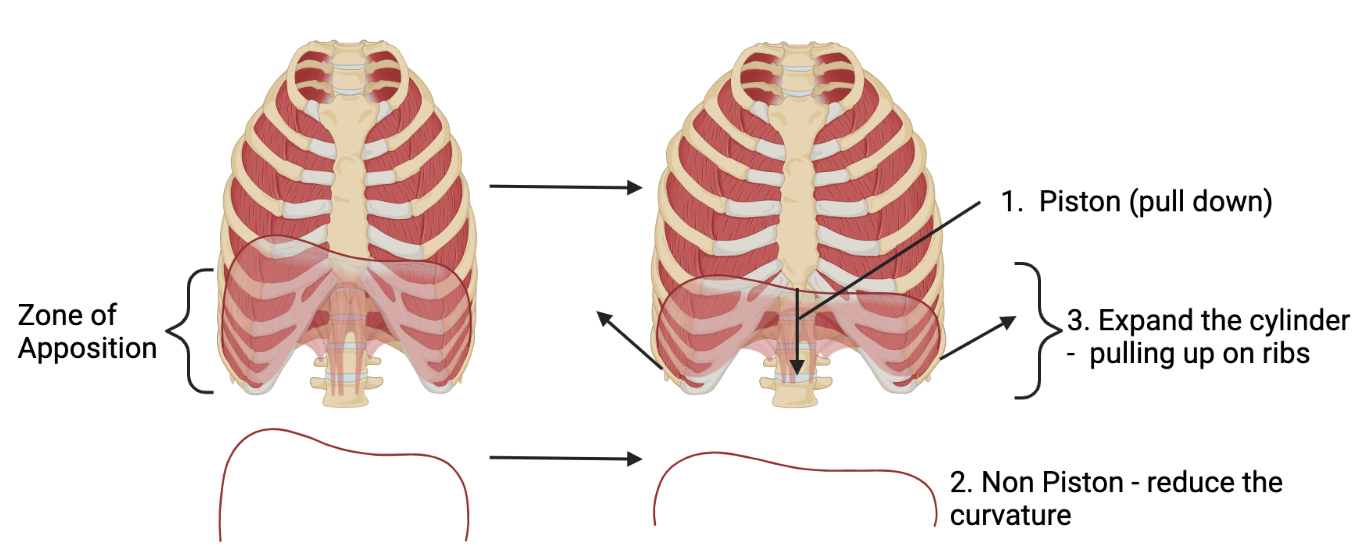
\includegraphics[width = 1.0 \linewidth]{./figure/ventilation/diaphragm.png}
    \caption{Three Actions of the Diaphragm to Expand the Thoracic Cavity \footnotesize{(Created in BioRender.com)}}
    \label{fig:diaphragm}
\end{figure}

There are many factors that influence how the above three actions that diaphragm mechanics contribute to inspiration. What is clear is that the larger the inspiratory volume, the more diaphragm activity is required and the likelihood that all three mechanical approaches are involved. The two most important factors influencing these mechanics are activity (which influences the amount of air that must be ventilated ($V_e$)); and posture. For example, in supine the "Expand the Cylinder" approach tends to dominate because abdominal mass reduces downward movement of the diaphragm which increases upward pull on the lower ribs.

\subsubsection{Intercostals \& Scalenes}

The exact coordination and involvement of the external and internal intercostals during breathing is complicated and most descriptions (including this one) is a simplification \cite{lumb_nunns_2020, de_troyer_respiratory_2005}. There are several contradictory sources about which set of intercostals are involved with inspiration vs. expiration \cite{lumb_nunns_2020, hall_guyton_2020}. To avoid those contradictions, and since there is little practical value to those arguments, we simply consider the intercostals and do not attempt to assign a particular breathing role to the external or internal sets. We rather consider both the internal and external as contributing to either lifting the ribs (for inspiration) or lowering the ribs (for expiration) from their axes at the costotransverse and costovertebral joints in the thoracic spine. We consider this based on motor coordination patterns \cite{gilbert_recognizing_2014}.

The inspiration motor coordination pattern for the intercostals starts with the activation of the scalenes. Scalenes are active even during quiet breathing. They stabilize the first rib. The first rib is then the anchor for each rib below it, in succession, to pull upward on the rib below it. They support, or pull up, rib 1. From this base of support the intercostals between rib 1 and 2 stabilize, or pull up, rib 2. From the base of support at rib 2, the intercostals between rib 2 and 3 stabilize, or pull up, rib 3. The pattern continues to rib 12 - the stabilized rib n, allows the intercostals between rib n and n+1 to stabilize, or pull up, rib n+1.

Based on the costotransverse and costovertebral joint axes, and in combination with attachment to the sternum, the upward movement of the upper ribs (1 - 6 or so), is described as "pump handle" which primarily includes a change in the anteroposterior (AP) diameter of the thoracic cavity. The upward movement of the lower ribs (7ish through 12) is described as "bucket handle" which primarily includes a change in the medial-lateral (ML) diameter of the thoracic cavity.

Even during quiet breathing there is active tension generated in the scalenes and intercostals, even if there is no movement of the ribs. These isometric contributions prevent inward movement of the ribs due to the drop in thoracic pressure by the diaphragm. In premature infants with underdeveloped intercostal muscles, or people with C5 to C8 spinal cord injury that have innervation of the diaphragm but do not have innervation of the intercostal muscles, thoracic paradox breathing mechanics can impair ventilation. Thoracic paradox includes a diaphragm piston like activation that reduces thoracic pressure and pulls the ribs inward which reduces the change in thoracic $V$ and limits ventilation. It is thoracic paradox because the thorax is not doing what is expected during inspiration. 

\paragraph{Question:} What is an abdominal paradox breathing and when might it occur?

\subsubsection{Accessory Inspiratory Muscles}
Accessory muscles are not active during normal breathing, but as ventilation increases there is a greater need to increase the thoracic cavity size, and therefore greater chest wall excursion (CWE).

Increasing the dimensions of the thoracic cavity requires more tension and range of contraction in the inspiratory muscles and can include recruitment of accessory muscles. Other reasons for accessory muscle activation may be when there are limitations in the primary muscles or when there are pulmonary conditions making ventilation less efficient. Accessory muscles include the sternocleomastoids, extensors of the vertebral column, pectoralis minor (and to a lesser extent major), trapezius and the serratus anterior and posterior muscles. For many of these muscles to serve an accessory role to inspiration the upper extremity must be stabilized so that tension in the muscle moves the thorax, not the limbs. In people with severe pulmonary disease that rely on accessory muscle activation for breathing, activities that use the upper extremities can be considerably limited.

\paragraph{Spinal Extension} increases thoracic cavity size. Think of the rib cage as an accordion. With spinal extension the accordion opens. Spinal extension (and the spinal extensors) is therefore an inspiratory accessory movement (and therefore spinal extensors are accessory muscles).


\subsection{Muscles of Expiration: Decrease Thoracic Cavity Volume}

\subsubsection{Intercostals}

The motor coordination pattern for using the intercostals to decrease thoracic cavity volume starts with the abdominal muscles (rectus abdominus, external and internal obliques). The abdominal muscles stabilize the lower rib cage so that intercostal contraction pulls down on the rib above it to reduce the size of the thoracic cavity (cylinder). This is the opposite coordination pattern of inspiration when the scalenes stabilized the first rib. 

\subsubsection{Abdominal Muscles}

The abdominal muscles have three roles in expiration (particularly forced expiration).

\begin{enumerate}
\item Stabilize the lower ribs so that intercostal activation pulls ribs down.
\item Pull the lower ribs down (they pull the lower ribs down much more than the scalenes can pull the first rib up - so the role of the scalenes for inspiration, while important, is really limited to stabilizing that first rib). The pulling down on the lower ribs significantly contributes to reducing the size of the thoracic cavity (the cylinder) and therefore the abdominals are a primary muscle of forced expiration.
\item Reduce abdominal cavity volume $\rightarrow$ increases abdominal cavity pressure $\rightarrow$ pushes up the relaxed diaphragm $\rightarrow$ reduces thoracic cavity volume and resets the piston (stretches the diaphragm for the next inspiration
\end{enumerate}

\subsubsection{Accessory Expiratory Movement}

As you probably figured out, if spinal extension is an accessory inspiratory movement then spinal flexion is an accessory expiratory movement. Of course, the abdominal muscles (collectively) are the spinal flexors and they are primary expiratory muscles, so they are not also accessory expiratory muscles. It is simply the case that if spinal flexion accompanies expiration, either intentionally to get as much air out as possible, or unintentionally due to the force of the abdominal muscles during expiration, then it is an expiratory accessory movement. Note: forced expiration that must include abdominal muscle activation but does not include spinal flexion, must involve spinal extensors to generate an equal, but opposite torque so that the spinal flexor muscles perform the three tasks they perform for expiration, but do not flex the spine.

\subsection{Pulmonary \& Pleural Pressures}
The discussion about the mechanics of ventilation have rightly assumed coherence between the lungs and the thoracic cavity. When the thoracic cavity increases volume, the lungs increase volume which increases the volume of the alveoli. When the thoracic cavity decreases its volume, the lungs decrease volume which decreases the volume of the alveoli. Under all normal circumstances these events are true. 

\paragraph{But....} the anatomical fact is that there is no direct connection between the lungs and the inner wall of the thoracic cavity. There is a space, it's a small space and it's filled with fluid, but it's a space. It is the pleural space and it is filled with pleural fluid. The lungs are lined with a lung pleural membrane and the thoracic cavity is lined with a thoracic pleural membrane. Between them is a thin space with pleural fluid. This arrangement allows the lungs to move within the thoracic cavity with relatively little friction (similar to the pericardial space and the pericardial fluid around the heart). 

To keep the lungs inflated and moving along with the thoracic cavity the pleural space is kept at a slightly negative pressure (negative in comparison to the atmosphere, and the atmosphere is taken as 0 cm of water ($cm H_2O$)\footnotemark\footnotetext{In ventilation physiology it is common to simply refer to the atmosphere as 0 which is a relative measurement based on the fact that when not breathing the atmosphere and alveoli pressures equilibrate and that for ventilation it is only differences in these pressures that matter. However, when calculating the partial pressures of gases, we consider the absolute atmospheric pressure which, at sea level, is 760 $mmHg$ (1033 $cmH_2O$)}. This is called the pleural pressure. The normal pleural pressure at the beginning of inspiration is about $-4 mmHg$, which is the amount of suction required to hold the lungs at their resting volume. During inspiration the thoracic cavity expands and the pleural pressure drops to approximately  $-7.5 mmHg$. These values are being shared simply to convey that they are slightly negative. 

\begin{figure}
    \centering
    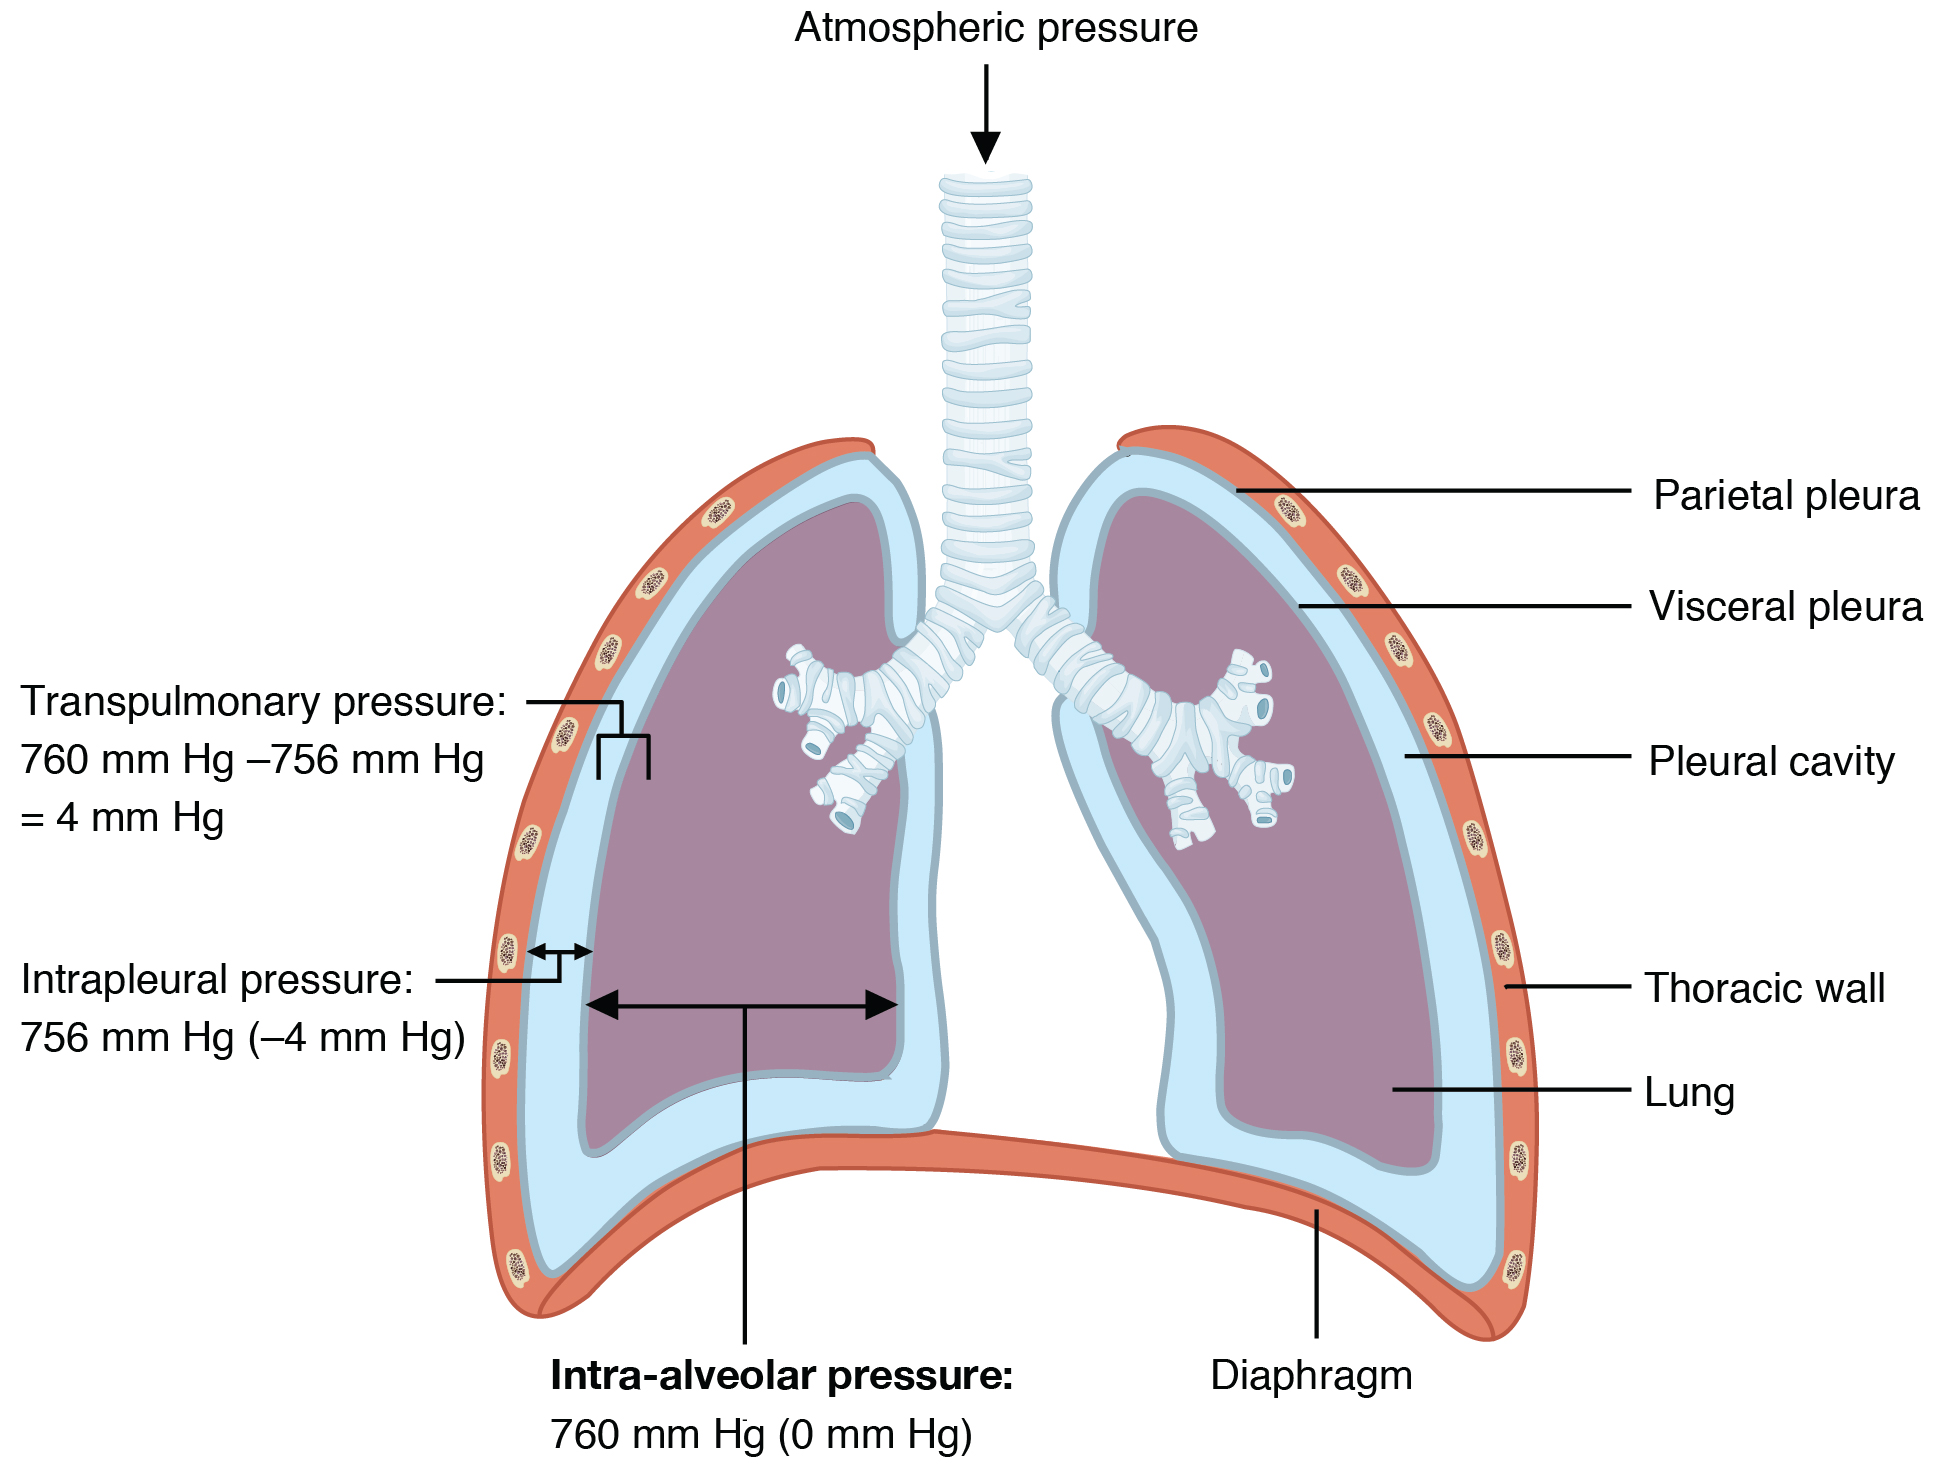
\includegraphics[width = 0.6 \linewidth]{./figure/ventilation/intrapulmonaryPressures.jpg}
    \caption{Intra Pulmonary Pressures \footnotesize{(OpenStax, CCBYSA4.0)}}
    \label{fig:intrapulmonaryPressures}
\end{figure}

During regular (resting $V_t$) expiration the lungs recoil and pull the thoracic cavity thus maintaining the negative pressure of the pleural space. Due to the movement of the thoracic cavity along with the lungs the pleural pressure returns to $-4 mmHg$.

During forced expiration the pleural pressures become slightly positive as the thoracic cavity pushes on the lungs to reduce their volume. The positive pleural pressure can result in a greater degree volume loss in alveoli, and reduction in the size of bronchioles and bronchi than due to the reduction in the volume of the thoracic cavity. In other words, during forced expiration the thoracic cavity directly reduces the lung size and this reduction is further influenced by a positive pleural pressure that also decreases lung airways and alveoli volume. This effect is more pronounced with a greater force for forced expiration because there is a higher positive pleural pressure.

\paragraph{Pneumothorax} is the collapse of a lung which can be precipitated by a loss of negative pleural pressure due to trauma. In certain trauma scenarios air may escape the lung and enter the pleural cavity resulting in positive pleural pressure which collapses the lung. This situation is called a tension pneumothorax and requires the positive pleural pressure to be removed with a tube placed into the chest (chest tube). Chest tubes are commonly used after thoracic surgery (any surgery that opens the thoracic cavity) to prevent the accumulation of edema and also to maintain negative pressure via suction to keep the lungs inflated.

\paragraph{Pleural Effusion} is the accumulation of fluid in the pleural space which then compresses the lung.

\subsubsection{Lung Compliance} 

Lung Compliance is the change in lung volume for each unit of change in transpulmonary pressure. Transpulmonary pressure is the difference between the alveolar and pleural pressures. For example (and not to memorize), the normal total compliance of both lungs together in a healthy adult is about 200 $mL/cm H_2O$ (for each 1  $cm H_2O$ change in pressure there would be a 200 $mL$ change in volume). 
Lung compliance depends on the elastic recoil forces of the lung. The elastic recoil forces are determined by the elastin and collagen fibers and the surface tension of alveoli. Increased elastic recoil forces (including increased surface tension) decreases compliance. For example, if there is more elastic recoil the compliance may be 100 $mL/cm H_2O$ which means only 100 $mL$ of volume for a 1 $cm H_2O$ change in pressure).

\paragraph{Surface tension of the alveoli} is the tendency for the $H_2O$ molecules on the surface to attract each other and contract (reduce the volume) of the alveoli. This force is strong enough that it can result in the collapse of the alveoli. Collapse of alveoli is called atelectasis, and one of the primary reasons patients are encouraged to do deep breathing and start moving around early after surgery (which keeps PTs in acute care  hospitals busy) is to prevent, or reverse, atelectasis.

\paragraph{Surfactant} is secreted by alveolar epithelial cells and reduces the surface tension in the alveoli substantially (to about $\frac{1}{12}$ the surface tension without surfactant). This substantial reduction in surface tension helps to maintain normal lung compliance, and to keep alveoli open. Since there is still some surface tension alveoli have a tendency to get smaller over time (hours). As alveoli get smaller there is less surface area which leads to increased surface tension because surfactant is pushed out of the alveoli. This reduces compliance and increases the risk of collapse (atelectasis). A protective mechanism against this is an occasional deep breath (cycles in inspiratory volume) open the alveoli which allows surfactant to move back into the alveoli. Following surgery with general anaesthesia there is a reduced drive to breath which lowers breathing volume and reduces the occasional deep breath from occurring (yawns, sighs, or just from moving around). This places individuals at a higher risk of atelectasis, which causes problems with oxygenation and also can be a precursor to pneumonia. Another effect is that clearing the anaesthesia from the body is facilitated by respiration and ventilation, so impaired respiration slows down clearance of the anaesthetic that is impairing the drive to breathe more deeply in the first place. Therefore, it is common for post operative rooms and surgical units to regularly encourage deep breathing as patients recover from surgery with exercises and even biofeedback such as an incentive spirometer (provides visual feedback about how much volume has been inhaled). 

\paragraph{Neonatal Respiratory Distress Syndrome (NRDS)} occurs in premature infants that have not yet started to create and release surfactant. They have very low lung compliance and require mechanical ventilation for breathing. But even the mechanical ventilation is challenging because as the ventilator pushes a sufficient volume of air into the lungs for ventilation the pressure rises substantially, because of the low compliance, which can then cause pressure trauma (baro-trauma) and worsen the overall pulmonary situation with lung inflammation. The availability of and delivery technologies for artificial surfactant has significantly improved the outcomes in such situations.

\section{Ventilation / Perfusion Matching}

Ventilation serves respiration. This is not the only function of ventilation, but it is certainly a primary function. For ventilation to serve respiration it must result in alveolar ventilation, $V_A$. And most of that fresh $V_A$ must match pulmonary capillary perfusion ($Q$). $V/Q$ matching requires minimizing the situations that result in mismatching. There are two general situations that result in mismatching, dead space ventilation ($VD$) and right-left pulmonary shunt (RL shunt). Minimizing these situations involves the pulmonary circulation regulation discussed in Chapter \ref{chp:blood_oxygen} on Respiration in the section on the Regulation of Pulmonary Circulation. This is a good time to review that section of the Respiration Chapter if needed.

\subsection{Dead Space Ventilation ($VD$)}

As introduced in the Ventilation Overview section, there are three classifications for dead space: anatomical, alveolar and physiological.  
\vspace{3mm}
To summarize:
\begin{itemize}
       \item Anatomical dead space ventilation ($V_D_{ana}$) is air ventilated but that does not make it into alveoli, $V_D_{ana} = V_e - V_A$
    \item Alveolar dead space ventilation ($V_D_{alv}$) occurs in alveoli that receive ventilation but do not receive alveolar circulation
    \item Physiological dead space ventilation ($V_D$) is the sum of anatomical and physiological dead space, $V_D = V_D_{ana} + V_D_{alv}$
\end{itemize}

\paragraph{Anatomical dead space ventilation ($VD_{ana}$)} was discussed in the section on Airways, since it is the volume of air that is ventilated but remains in the conductive zone of the airways (does not make it to the alveoli). $V_D_{ana}$ is minimized by regulating, and optimizing, the breathing pattern volume and rate. Larger volumes certainly reduce $V_D_{ana}$, but if volumes are too large then the work of breathing becomes more difficult for three reasons:

\begin{enumerate}
    \item Inspiratory muscles shorten and it's more difficult to generate the required active tension based on their length - tension curve.
    \item The thoracic cavity increases and starts to resist further increases due to passive tension so the muscles must work harder (at a time that it is harder for them to work based on #1)
    \item Lung compliance starts to decrease because as lungs expand the lung elastic recoil forces (like passive tension) increase (and recall that lung elastic forces are inversely proportional to compliance)
\end{enumerate}

For all of those reasons - optimizing breathing pattern requires a balance between higher volumes and lower rates, which minimize $V_D_{ana}$ but increase the word of breathing; and lower volumes and higher rates, which maximize $V_D_{ana}$, but lower the work of breathing.

\paragraph{Alveolar dead space ventilation ($V_D_{alv}$)} is minimized by the regulation of pulmonary circulation. Pulmonary arterioles dilate in areas with increased $O_2$ and constrict in areas with decreased $O_2$. They also dilate in alveoli receiving fresh ventilation taken in through the nose that has had nitric oxide (NO) since NO is a vasodilator.

\paragraph{Perfusion Zones} exist throughout the lung because gravity, and therefore body position, influences distribution of $V_D_{alv}$ and perfusion. Furthermore, the distribution of alveolar residual volume influences perfusion as described below. The lungs can be broken into three perfusion zones that are based on gravity (See Figure \ref{fig:perfusion_zones}).
\vspace{2mm}
The zones are:
\begin{enumerate}
    \item Upper Zone: receives less new $V_A$ because during expiration the alveoli do not decrease in size as much, so there is less overall change in their volume and less overall change in air ventilated; receives less $Q$ because the pulmonary circulation is a lower pressure system so its arterial flow is influenced more by gravity (harder to pump blood up) as well as the residual volume of the alveoli. The Upper Zone has more of the $FRC$ and $RV$. With a higher residual volume of air in the alveoli the pulmonary capillaries are compressed (in addition to the constriction of the arterioles due to lower $O_2$ delivery.
    \item Middle Zone: receives more $V_A$ than the Upper, but less than the Lower Zones; and more $Q$ than the upper, but less than the Lower. There is a lower alveoli residual volume than in the Upper zone, and more than in the Lower zone.
    \item Lower Zone: receives more new $V_A$ because during expiration the alveoli decrease in size substantially so there is more overall change in their volume and more overall ventilation; receives more $Q$ because the pulmonary circulation is influenced by gravity. The Lower Zone has less of the $FRC$ and $RV$. With less residual volume the pulmonary capillaries are not compressed, and in combination with the dilated arterioles (due to the higher $O_2$ values from the increased ventilation) $Q$ is greater than the other zones.
\end{enumerate}
\vspace{3mm}

\begin{figure}[!h]
    \centering
    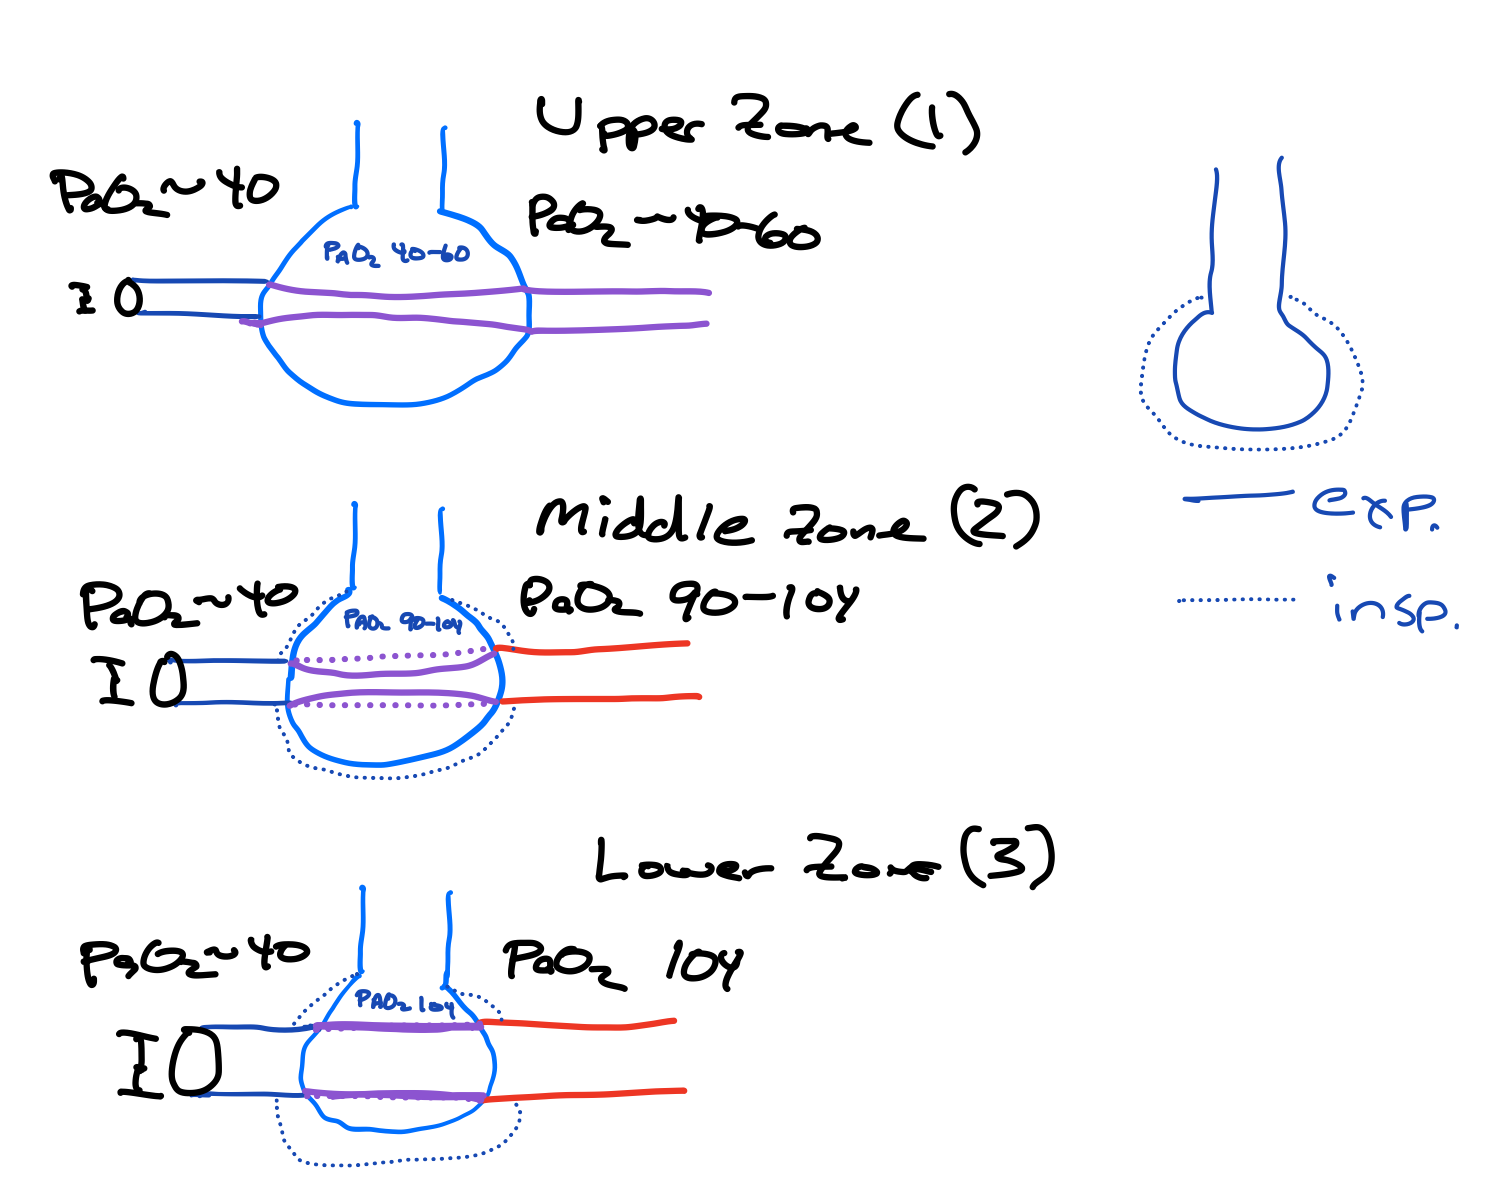
\includegraphics[width=0.75 \linewidth]{./figure/ventilation/perfusion_zones.png}
    \caption{Perfusion Zones (Draft)}
    \label{fig:perfusion_zones}
\end{figure}

The combination of pulmonary circulation regulation and pulmonary zones whereby gravity influences $V$ and $Q$ results in normal resting $V/Q$ matching of approximately 80\%. This is an empirical figure based on the use of a ventilation/perfusion lung scan, also called a $V/Q$ scan.  The imaging uses medical isotopes to evaluate the circulation of air and blood within the lungs to determine the ventilation/perfusion matching. 

\paragraph{} \textit{Pulmonary Embolism} is a blood clot that travels to and lodges in a pulmonary artery or arteriole that cuts off blood blow to a section of alveoli capillary circulation. This is a life threatening situation that immediately and substantially causes alveolar dead space and thus physiological dead space, reducing the $V/Q$ matching, reducing respiration and therefore $P_aO_2$.


\paragraph{Physiological Dead Space ($V_D$)} is the sum of anatomical and alveolar dead space and can be estimated with the Bohr Equation:

\begin{equation}
    VD = V_t \times \frac{(P_aCO_2 - etCO_2)}{P_aCO_2}
    \label{eq:bohr}
 \end{equation}
 
$etCO_2$ is the end tidal partial pressure of $CO_2$ measured at the nose at the end of expiration.

\paragraph{For example:} If $V_t$ is 500 $mL$, $P_aCO_2$ is 40 $mmHg$, and $etCO_2$ is 35 $mmHg$ then $V_D$ is estimated as 62.5 $mL$. The units are in $mL$ because the $V_t$ is in $mL$ and it is multiplied by a ratio which is unitless since the $P_aCO_2$ and the $etCO_2$ are both in $mmHg$.

\paragraph{Question:} Figure out the $V_D$ if $V_t$ is 300 $mL$, $P_aCO_2$ is 50 $mmHg$, and $etCO_2$ is 30 $mmHg$. How does this compare with the above example? 

\paragraph{Question:} Figure out the $V_D$ if $V_t$ is 300 $mL$, $P_aCO_2$ is 40 $mmHg$, and $etCO_2$ is 15 $mmHg$. How does this compare with the above examples?

\paragraph{Advanced concept:} Why does this equation work? (Not necessary, just if you're looking for more challenge and something to do on a Friday night.)

\subsection{Right-Left Shunt}

Another situation that can result a $V/Q$ mismatch is a right-left (RL) shunt. When alveolar dead space causes a mismatch it is because ventilated alveoli do not receive any (or enough) perfusion. A RL shunt is the opposite situation. Alveoli that do not have ventilation, or are under ventilated, receive blood flow. Because this blood flow does not exchange gases with the alveoli (because the alveoli does not have ventilation), the right sided blood (venous blood) returns unchanged and joins with the left sided blood (arterial blood). 

The simplest cause of a RL shunt is not breathing (apnea). With apnea the alveoli still have air. However, since the alveoli equilibrate with blood passing through they quickly, without $V_A$, have the same amount of $O_2$ and $CO_2$ as venous blood. This results in elevated $P_aCO_2$ and reduced $P_aO_2$ that worsen with prolonged apnea. While holding your breath is apnea, we should reserve the term apnea for pathological causes of not breathing. Voluntary breath hold to the point of lowering $P_aO_2$ is very difficult so is not as good of an example of a RL shunt.

Pathological causes of RL shunts include anything that results in hypoventilation (reduced $V_A$), including conditions that fill the alveoli with something other than ventilated air. For example, pulmonary edema, mucus from pneumonia, inflammation with any pulmonary inflammatory condition such as COVID (which can also cause pneumonia). Chronic pulmonary conditions such as emphysema and bronchitis increase the $RV$ which increases the number of alveoli getting blood flow but not new ventilation, a RL shunt.

\subsubsection{$V_D$ \& RL Shunt}

There is a bit of an inverse relationship between $V_D$ and RL shunt. Across all the alveoli-capillary interaction space between both lungs, and assuming ventilation and blood flow are both occurring, then any alveoli getting ventilation and not perfusion ($V_D$) means there are other alveoli getting perfusion and not ventilation. An extreme - and purely academic - example would be if all ventilation went to the right lung; and all blood flow went to the left lung. In this situation the overall $V/Q$ matching is 0\%. The right lung is completely dead space ventilation $V_D$; and the left lung is a complete RL shunt.


\subsection{A-a Gradient}

The A-a gradient is the drop off that occurs between the partial pressure of $O_2$ from fully ventilated alveoli ($P_AO_2$) to the partial pressure of $O_2$ in mixed arterial blood ($P_aO_2$). The $P_AO_2$, at sea level with a normal fraction of inspired oxygen ($F_iO_2 = 0.21$) is taken as 104 $mmHg$. This blood mixes with blood from other regions of the lung as it travels back to the left atrium. In addition to the venous blood from the bronchial pulmonary circulation, there is blood from normally occurring RL shunts given the normal resting $V/Q$ matching of 80\% (20\% mismatching). Therefore, we should not be surprised that the normal $P_aO_2$ is less than 104 $mmHg$ of $P_AO_2$. This difference (approximately 104 - 95 = 9 mmHg) is the A-a gradient. The A-a gradient is proportional to the severity of a RL shunt (See Figure \ref{fig:aagradient}). In critical care situations the A-a gradient can be elevated even when a patient has a normal blood oxygen level because the $P_AO_2$ is elevated. 
For example, if a patient at sea level is on supplemental oxygen with an $F_iO_2 = 0.6$ (60\% oxygen), then the estimated $P_AO_2$ is 300 $mmHg$, and the A-a gradient even with a normal $P_aO_2$ would be 205, indicating substantial RL shunting.

\begin{figure}[!h]
    \centering
    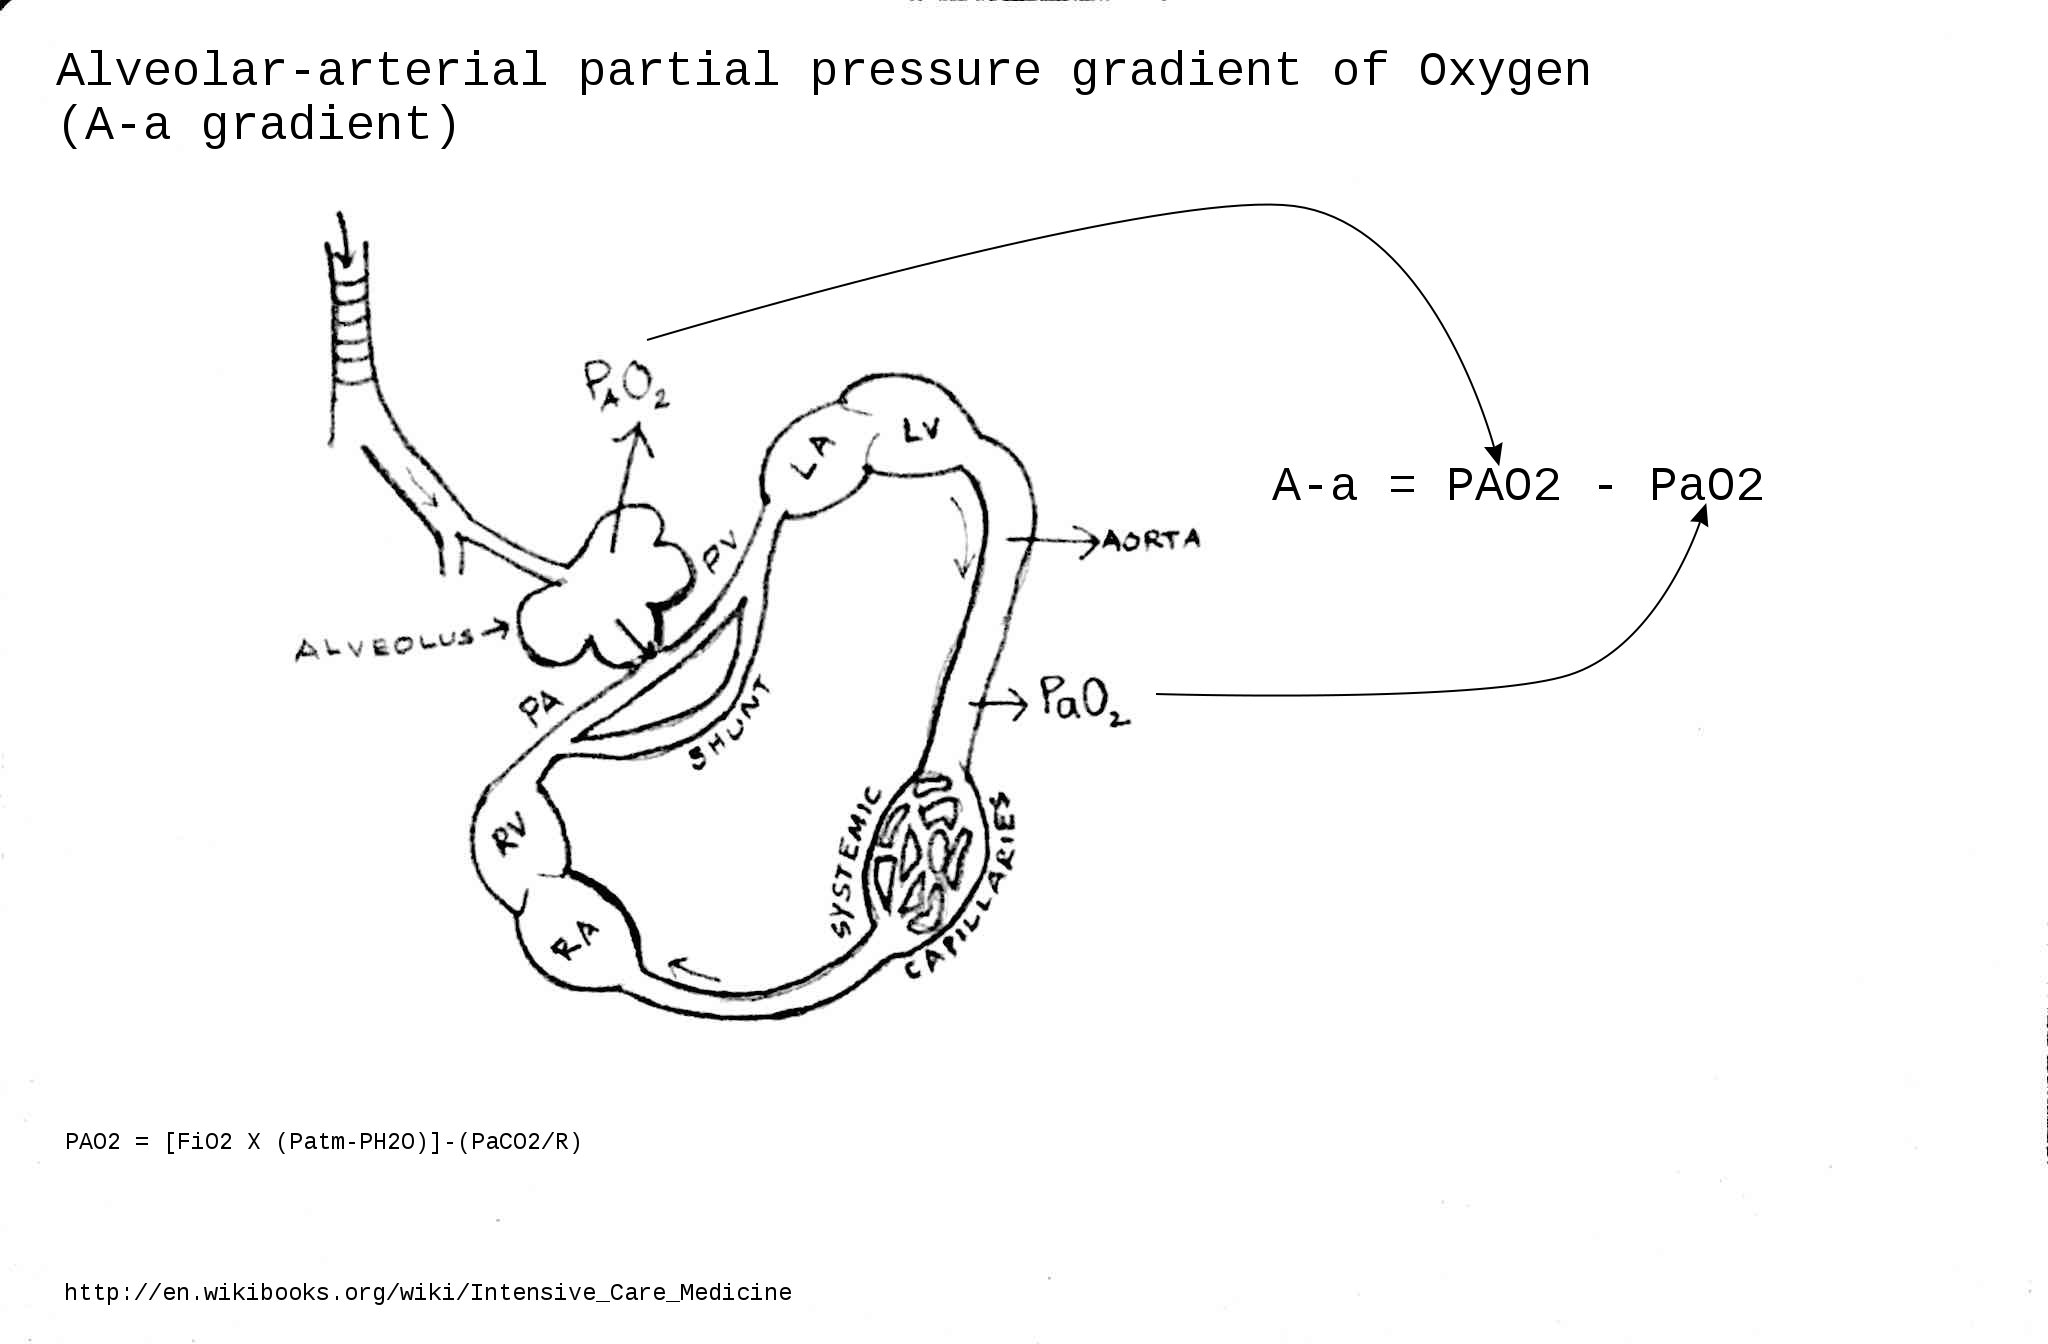
\includegraphics[width=1.0 \linewidth]{./figure/ventilation/aagradient.jpg}
    \caption{RL Shunt \& A-a Gradient \footnotesize{CCBYSA4.0, \href{https://commons.wikimedia.org/wiki/File:Intensivecaremedicine_aagradient.jpg}{WikiMedia Commons}}}
    \label{fig:aagradient}
\end{figure}


\section{Regulation}

Ventilation, including breathing volume, pattern and coordination, usually occurs without thought. However, the volume, pattern and coordination can be consciously controlled. Ventilation has automatic but voluntary control - like posture and gait and any learned movement. Ventilation (breathing) is the first movement people learn. Like any movements (or postures), there are many factors that can alter breathing from its optimal performance.

\textbf{Ventilation volume ($V_e$)} is of volume ventilated in a time period (usually a minute). 

\textbf{Ventilation pattern} is the particular combination of tidal volume and respiratory rate to achieve $V_e$. Since $V_e = RR \times V_t$, where $RR$ is the rate in breaths per minute and $V_t$ is the tidal volume in $mL$, there are numerous combinations possible to achieve the same $V_e$. The combination of $RR$ and $V_t$ is the ventilation (breathing) pattern (also the pattern of breathing). 

\textbf{Ventilation coordination}, also referred to as \textbf{breathing mechanics}, refers to the various combinations of coordinated muscle activation, or the various mechanical changes to the thoracic cavity that different coordination of muscle activation produces. A major determinant of ventilation coordination (breathing mechanics) is how much diaphragm activation is involved with ventilation. More diaphragm activation results in "belly breathing", whereas less diaphragm results in "chest breathing", by necessity and activation of the intercostals and possibly the accessory muscles. Each of these ventilation coordination (breathing mechanics) can produce the same $RR$ and $V_t$, though chest breathing has a limit on the range of $V_t$.

\paragraph{} In Figure \ref{fig:breathing_patterns} the relationship between $V_t (mL)$ (on the x-axis) and $V_e (mL/min)$ (on the y-axis) with three different $RRs$ is depicted. Each $V_t$, $RR$ combination is a different breathing pattern. Since breathing mechanics that utilize the diaphragm allow a larger $V_t$, those mechanics are capable of the full range of the $V_t$ (x-axis). When not using the diaphragm there is a limit to the $V_t$ (x-axis). In Figure \ref{fig:breathing_patterns} the limit to $V_t$ when not using the diaphragm is taken as 300 $mL$ (dotted orange vertical line). If the metabolic needs of the body require $V_e$ of 4000 $mL/min$ (yellow horizonal line) then diaphragm breathing mechanics can achieve this with a lower RR and greater $V_t$. However, chest breathing mechanics limits the possible breathing patterns to those with a $V_t$ of less than 300 $mL$, which requires a greater $RR$.

\begin{figure}
    \centering
    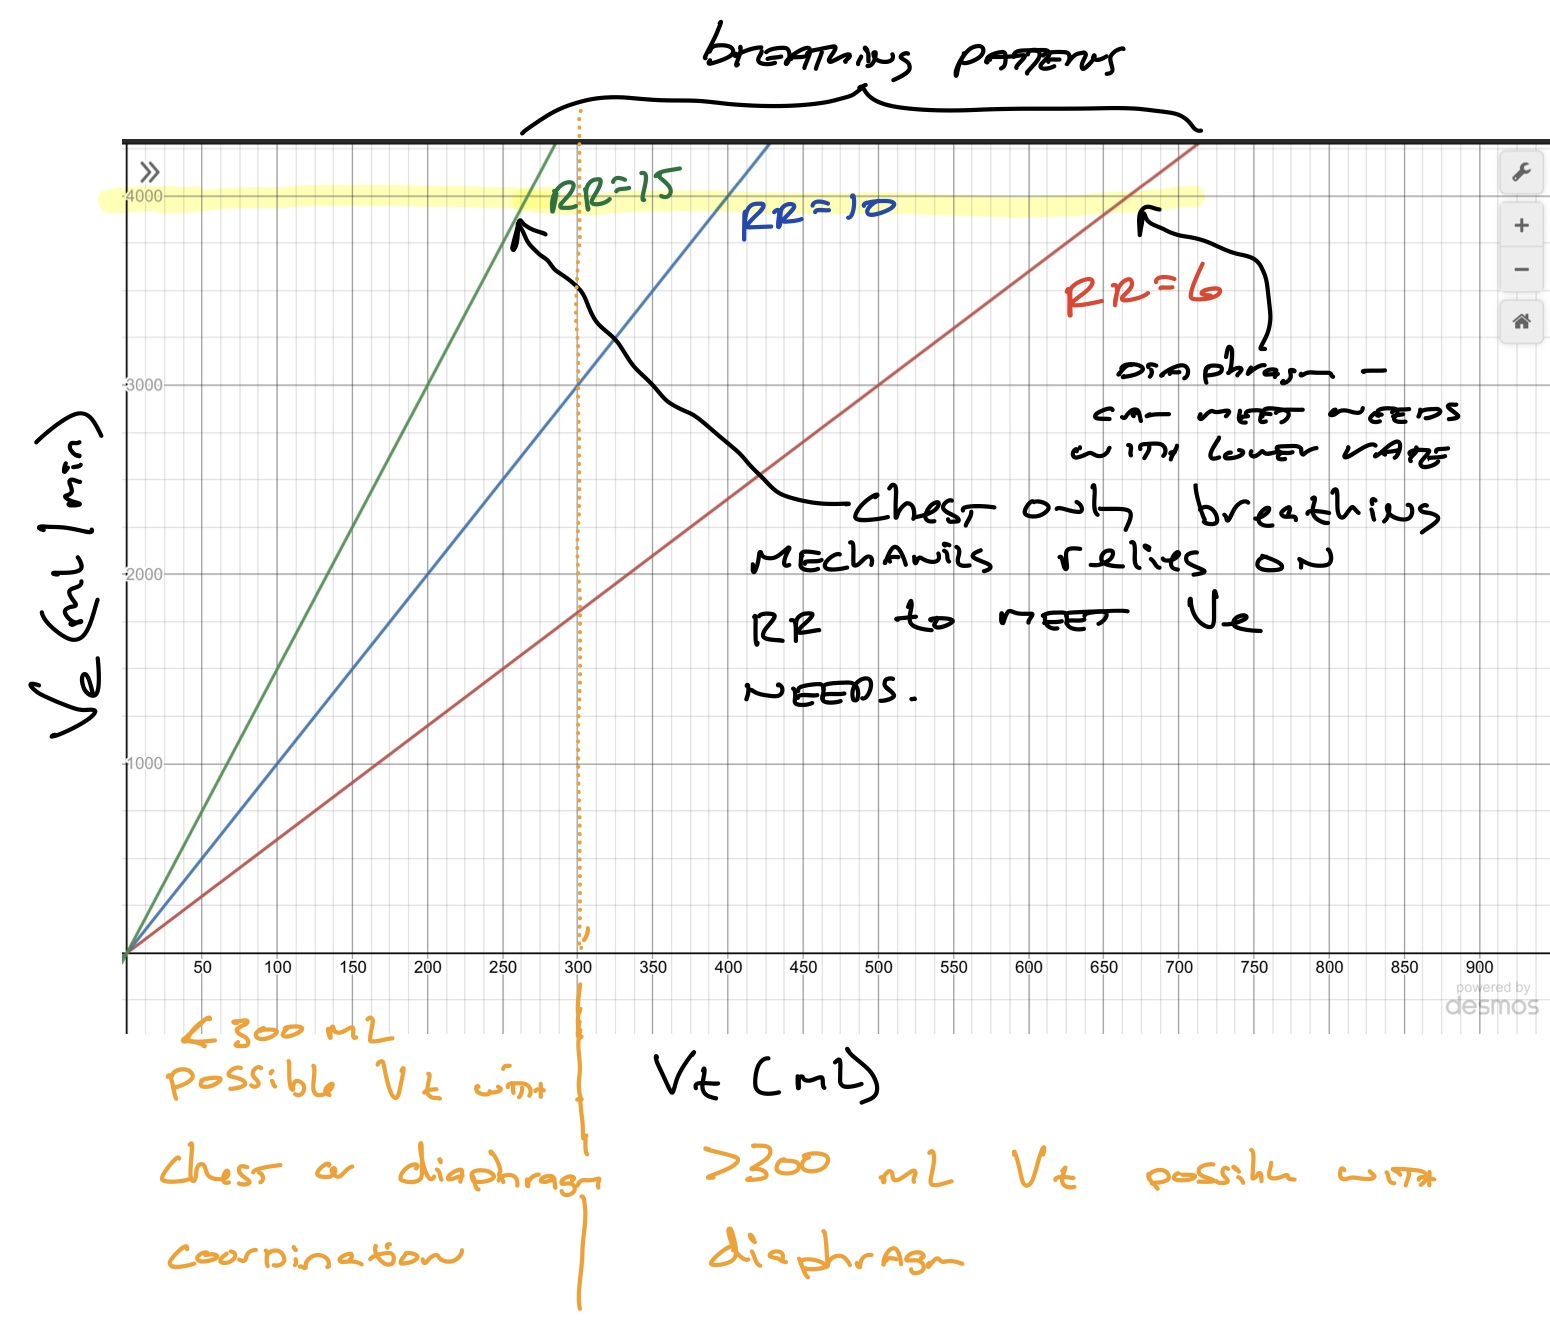
\includegraphics[width=1.0 \linewidth]{./figure/ventilation/breathing_patterns.jpg}
    \caption{Breathing Pattern Combinations at RR = 6, 10 or 15 (Draft)}
    \label{fig:breathing_patterns}
\end{figure}

\paragraph{Challenge Question:} In Figure \ref{fig:breathing_patterns} the need for $V_e$ is taken as 4000 $mL$. In this example, that volume is based on an assumed metabolic need. Since the metabolic need is actually met by $O_2$ that gets into alveoli ($V_A$), and since $V_A$ is influenced by anatomical dead space ($V_D_{ana}$), and since anatomical dead space is related to the breathing pattern (combination of $RR$ and $V_t$), would the actual $V_e$ need be the same between the $RR$ = 6 vs. the $RR$ = 15 pattern? How would anatomical dead space factor in and change the model assumptions in Figure \ref{fig:breathing_patterns}? Hint: Consider your answer to the question in the Airway Section on Anatomical Dead Space.

\subsection{Ventilation Control Centers}

Neurons that innervate the muscles of the respiratory system are responsible for controlling and regulating pulmonary ventilation. The major brain centers involved in pulmonary ventilation are the medulla oblongata (medullary respiratory center) and the pons (pneumotaxic center). The medullary respiratory center is responsible for the rhythm of breathing and automatic ventilation. The pneumotaxic center controls the rate and depth of ventilation. The cerebral cortex sends impulses directly to the motor neurons of the ventilatory muscles which allows for voluntary control of ventilation.

\subsection{Factors That Affect Ventilation} 

The medullary respiratory center and the pneumotaxic center adjust $V_t$ and $RR$ in response to afferent input.  The overall response patterns are dose-response, negative-feedback. The greater the stimulus, the greater the response. Increasing stimuli results in higher $RR$ and greater volume with $V_t$. These both typically include forced expiration.  Multiple factors are involved in stimulating the the centers to adjust. Major factors are the concentration of carbon dioxide in the arterial blood ($P_aCO_2$), and the pH, as sensed by chemoreceptors. A central chemoreceptor is one of the specialized receptors that are located in the brain and brainstem, and a peripheral chemoreceptor is one of the specialized receptors located in the carotid arteries and aortic arch. Increased $P_aCO_2$ and decreased pH (acidity), stimulate the respiration centers to increase $V_e$ through some combination of increasing $RR$ and $V_t$, with some combination of muscles (coordination, mechanics). Reduced $P_aCO_2$ and increased pH (alkaline), reduces stimulation and therefore reduces $V_e$.

There are chemoreceptors for $O_2$, and with hypoxia, $P_aO_2$ of less than 60 mmHg, these receptors are activated. The lower the $P_aO_2$ the stronger the stimulus. However, under normal circumstances the $P_aO_2$ is so far above the threshold for $O_2$ chemoreceptor stimulation they are rarely involved in the regulation of ventilation. If ventilation was reduced enough for hypoxia, then the increase in $P_aCO_2$ would be substantial enough to have strongly stimulated the $CO_2$ chemoreceptors to increase ventilation. To voluntarily allow hypoxia through breath hold, a period of hyperventilation that substantially reduces $P_aCO_2$ is necessary. This allows prolonged breath holding and enough time for $P_aO_2$ to drop. That hyperventilation, hypocarbia (low $P_aCO_2$) situation, is the underlying principle for what is popularly referred to as "Wim Hof Breathing." It can be used to create therapeutic exposures to intermittent hypoxia.

\subsection{Emotional \& Feed Forward Regulation}
The hypothalamus and other brain regions associated with the limbic system also influence breathing by interacting with the respiratory centers. These regions are responsible for changes in ventilation related in response to fight-or-flight, emotions, pain, and temperature. For example, an increase in body temperature causes an increase in respiratory rate. Feeling excited or the fight-or-flight response results in an increase in $V_e$. These responses, particular the fight-or-flight response act as feed forward regulation. Ventilation increases prior to an increase in $P_aCO_2$ with exercise because before $P_aCO_2$ has a chance to increase, ventilation has already increased.

\subsection{Protective Reflexes}

Protective reflexes such as coughing, sneezing, bronchoconstriction, mucus secretion and mucociliary activity respond to irritants such as smoke, dust or larger particles (larger than $O_2$ and $CO_2$). These coordinated reflexes work together to capture and expel irritants and potentially harmful pathogens.

\subsection{$CO_2$ Retainers - $O_2$ Drive for Breathing}

The combination of pulmonary diseases classified as chronic obstructive pulmonary disease (COPD) are progressive chronic conditions. In severe to end-stage COPD, among other things, there is chronically elevated $P_aCO_2$ that creates respiratory acidosis and metabolic compensation. The chronically elevated $CO_2$ and reduced pH can result in down regulation of the chemoreceptors to these stimuli. In these situations, $P_aO_2$ chemoreceptors are utilized to regulate $V_e$. A consequence of this situation is that $P_aO_2$ must be near hypoxia to increase ventilation. If someone in this situation is provided with too much supplemental $O_2$, which increases their $F_iO_2$, then their ventilation will decrease and their $P_aCO_2$ will increase further, to potentially dangerously toxic levels.

\section{Practice Connections}

Abridged for the sake of time.....

\subsection{Intermittent Hypoxia}

Intermittent hypoxia can have positive or negative consequences. When uncontrolled and very frequent (such as with sleep apnea) the consequences tend to be negative. With sleep apnea, there are frequent episodes of intermittent hypoxia that disturb sleep. Therefore, it is difficult to separate the consequences into those related to the hypoxia and those related to sleep deprivation.
Intermittent hypoxia - when controlled and not as frequent - is a stimulus (much like the fact that exercise is a healthy stimulus, whereas chronically performing heavy physical labor is unhealthy (or even just over exercising $\rightarrow$ over-training). Benefits of intermittent hypoxia include aerobic adaptations and brain cell stimulus \cite{navarrete-opazo_therapeutic_2014, verges_hypoxic_2015}.

\subsection{Pulmonary Function Tests - Forced Expiratory Maneuver}

The Forced Expiratory Maneuver (FEM) of Pulmonary Function Tests (PFTs) includes a full inspiration (until reaching total lung capacity ($TLC$)), followed by a forced expiration to expire as much air as fast as possible with the goal of expiring air until reaching the residual volume ($RV$). Subjects are usually seated for testing, but they are allowed to extend their spine during the full inspiration and flex their spine during the full, forced expiration. There are several measurements that are made from this single test. But, the two most important measurements for the physical therapist to recognize from an FEM of a PFT are the forced vital capacity ($FVC$) and the forced expiratory volume in 1 second ($FEV_1$). They are both measured in liters ($L$). 
Forced vital capacity ($FVC$) is an estimate of the vital capacity $VC$ and with healthy lungs $FVC = VC$. Forced expiratory volume in 1 second ($FEV_1$) is influenced by both expiratory volume and expiratory flow. The ratio of these two measures, the $FEV_1/FVC$ considers whether a reduction in $FEV_1$ is due to a reduction in $FVC$ (volume) or expiratory flow. When expiratory flow is normal: $FEV_1/FVC \approx 0.75$. The lower the $FEV_1/FVC$, the more substantial the limitation in expiratory flow.

\subsection{Ventilatory Muscle Testing}

There are numerous ways to test (and quantify) ventilatory muscle strength and endurance. The most common approach is the maximal inspiratory pressure (MIP) and the maximal expiratory pressure (MEP). MIP and MEP are isometric tests performed when the respective muscles are in their lengthened position. 
MIP testing is performed at residual volume ($RV$). The subject attempts to breath in as strongly as possible on a tube connected to a device that can measure negative pressure. There can be a small air leak to prevent the use of facial muscles from contributing mouth pressure to the negative pressure generated. 
MEP testing is performed at total lung capacity ($TLC$). The subject attempts to breath out as strongly as possible on a tube connected to a device that can measure pressure. There can be a small air leak to prevent the use of facial muscles from contributing mouth pressure to the positive pressure.
Even though MIP and MEP are isometric tests of pressure they are highly correlated with other approaches to measuring both ventilatory muscle strength and endurance. As with any muscle testing, care must be taken to ensure proper muscle coordination and activation. For example, when being asked to generate a strong inspiratory effort subjects commonly associate what they are being asked to do with a big breath and they associate big breaths with upper chest and accessory muscle use. If the tester wants an estimate of diaphragm strength, care must be taken to prepare the subject, and provide feedback to encourage diaphragm activation as opposed to upper test and accessory muscles. For example, establishing that subjects understand the request to breathe in with their diaphragm even before attempting the test. And then repeating whatever instructions led to a diaphragm activation while doing the test (i.e., "Breathe in forcefully, starting from deep in your lungs, starting the movement with your abdomen which should move outward while you breathe in.")

\subsection{Ventilatory Insufficiency Patterns}

There are two major ventilatory insufficiency patterns. 

\begin{itemi}
\item Obstructive pattern: Difficulty getting air out of the lungs during expiration due to airway resistance and bronchiole collapse. This pattern includes increased $RV$, increased $FRC$ and decreased $VC$. PFT's include reduced $FEV_1$ and $FVC$ and a reduced $FEV_1/FVC$ ratio, which means $FEV_1$ decreases more than $FVC$ because expiratory flow is significantly reduced.
\item Restrictive pattern: Difficulty getting air into the lungs for any reason (intra-pulmonary reasons are within the lungs such as pneumonia or fibrotic changes; extra-pulmonary reasons are outside of the lungs such as pleural effusion, chest wall changes or diaphragm weakness). $FEV_1$ and $FVC$ are decreased proportionally, $FEV_1/FVC$ ratio is normal, which means ($FEV_1$) is reduced because of an overall lower volume, not because of a reduction in expiratory flow.
\end{itemi}

Chronic pulmonary conditions such as emphsyema and bronchitis are termed chronic obstructive pulmonary disease (COPD) because they have an obstructive pattern. The increase in $RV$ eventually changes the anatomy of the thorax, which changes the mechanics of the inspiratory muscles. Therefore, even though there are expiratory flow limitations (reduced $FEV_1/FVC$), there is also a reduction in maximal inspiratory pressure (MIP) which contributes to the shortness of breath and activity intolerance. The increased $RV$ also results in substantially under ventilated alveoli (reduced $V_A$), which leads to substantial right-left shunt, which leads to substantial $V/Q$ mismatching, and therefore substantial problems with respiration that include both decreased $P_aO_2$ and increased $P_aCO_2$.

Asthma is a chronic condition that has acute obstructive episodes. Sometimes it is classified as a chronic obstruction, but this should only be the case when there actually is chronic obstruction (chronically reduced $FEV_1/FVC$ ratio).

\paragraph{Too much to say.....,} and so little time. Need to wrap up this chapter.

\section{Summary}
Ventilation is the movement of air into and out of the lungs and involves activation of skeletal muscles that change the shape of the thoracic cavity. This is always an active tension process for inspiration, and is usually a passive tension process for expiration. Forced (or additional) expiration requires active tension. 
Alveolar ventilation is the movement of air into and out of the alveoli. Alveolar ventilation that includes pulmonary perfusion (circulation) is involved in respiration. Ventilation that does not reach alveoli is called anatomical dead space ventilation. Alveolar ventilation that does not receive sufficient pulmonary circulation is called alveolar dead space ventilation. Physiological dead space (or just dead space) is the sum of anatomical and alveolar dead space. Pulmonary circulation that goes to alveoli not receiving sufficient ventilation is a right-left shunt. Dead space and right-left shunt reduce $V/Q$ matching (the opposite of $V/Q$ matching is $V/Q$ mismatching). 

\subsection{Next steps....}
Pull things together in Fick's equation; take the final exam; move onto the fall and come back for Digestion, Absorption \& Metabolism; as well as Myostasis (Muscle Integrity) in Exercise Prescription /& Nutrition....

\printbibliography[heading=subbibintoc]